\documentclass[sigconf]{acmart}

\fancyhf{} % Remove fancy page headers
%\fancyhead[C]{Anonymous submission \#399 to ACM CCS 2022} % TODO: replace 9999 with your paper number
\fancyfoot[C]{\thepage}

% \setcopyright{none} % No copyright notice required for submissions
\acmConference[ACM CCS 2022]{ACM Conference on Computer and Communications Security}{November 7-11, 2022}{Los Angeles, U.S.A.}

%\settopmatter{printacmref=false, printccs=true, printfolios=true} % We want page numbers on submissions

\newif\ifWorkInProgress
%\WorkInProgresstrue
\WorkInProgressfalse

\setcopyright{acmcopyright}
\copyrightyear{2022}
\acmYear{2022}
\acmDOI{XXXXXXX.XXXXXXX}

%-------------------------------------------------------------------------------
\usepackage[english]{babel}
\usepackage[utf8]{inputenc}
\usepackage{etoolbox}

%---- Math
\usepackage{dsfont}
\usepackage{mathtools}
\usepackage{mathdots}
\usepackage{centernot}
\usepackage{xspace}
\usepackage{thm-restate}

%---- Comments
\usepackage{totcount}
\usepackage{color}
\usepackage{verbatim}

%---- Images
\usepackage{graphicx}

%---- Layout
\usepackage{lscape}
\usepackage{float}
\usepackage{supertabular}
\usepackage{multirow}
\usepackage{longtable}
\usepackage{tabularx}
\usepackage{enumerate}
\usepackage{enumitem}
\usepackage{varwidth} %required for boxes
\usepackage[most]{tcolorbox} %and thus tikz
\usetikzlibrary{calc,arrows,positioning,decorations.pathmorphing,shapes,backgrounds,arrows.meta}
\usepackage{placeins}

%---- Refs & URLs
\PassOptionsToPackage{hyphens}{url}
\usepackage[capitalise,nameinlink,sort&compress]{cleveref}
\usepackage{subfig}

%---- Tables
\usepackage{makecell}

% ---- Acronyms
\usepackage{acro}

%%% Local Variables:
%%% mode: latex
%%% TeX-master: "../main"
%%% End:

%!TEX root = ../main.tex

%------------------------------
%  Do not add notation macros to this file
%  use notation.tex instead
%-------------------------------

%----- Theorems ----------------------------------------------------------------

%Non-LNCS theorem environments
%\newtheorem{theorem}{Theorem}
%\newtheorem{lemma}{Lemma}
%\newtheorem{corollary}{Corollary}
%\newtheorem{definition}{Definition}
%\newtheorem{example}{Example}

%This might work with amsthm
%\makeatletter
%\newtheorem{repeatthm@}{Theorem}{\bfseries}{\itshape}
%\newenvironment{repeatthm}[1]{%
%    \def\therepeatthm@{\ref{#1}}
%    \repeatthm@
%}
%{\endrepeatthm@}
%\makeatother


%LNCS related theorem environments
%\spnewtheorem*{theorem*}{Theorem}{\bfseries}{\itshape}
%\spnewtheorem*{theoremnn}{Theorem}{\bfseries}{\itshape}
%\spnewtheorem*{lemma*}{Lemma}{\bfseries}{\itshape}
%\newenvironment{claimproof}[1]{\par\noindent\underline{Proof}:\space#1}{\hfill $\blacksquare$}
\newenvironment{claimproof}[1]{%
	\def\squareforqed{$\blacksquare$}%
	\par\noindent\underline{Proof}:\space#1%
}{}
%\spnewtheorem*{definition*}{Definition}{\bfseries}{\itshape}
%\spnewtheorem{fancyclaim}{Claim}{\bfseries}{\itshape}
%\renewcommand{\qed}{\strut\hfill$\blacksquare$}

%This only works with LNCS!
% \makeatletter
% \spnewtheorem{repeatthm@}{Theorem}{\bfseries}{\itshape}
% \newenvironment{repeatthm}[1]{%
%     \def\therepeatthm@{\ref{#1}}
%     \repeatthm@
% }
% {\endrepeatthm@}
% \spnewtheorem{repeatlem@}{Lemma}{\bfseries}{\itshape}
% \newenvironment{repeatlem}[1]{%
%     \def\therepeatlem@{\ref{#1}}
%     \repeatlem@
% }
% {\endrepeatlem@}
% \spnewtheorem{repeatcor@}{Corollary}{\bfseries}{\itshape}
% \newenvironment{repeatcor}[1]{%
%     \def\therepeatcor@{\ref{#1}}
%     \repeatcor@
% }
% {\endrepeatcor@}
% \makeatother
\theoremstyle{definition}

\theoremstyle{plain}

\theoremstyle{remark}
\newtheorem{remark}{Remark}
\newtheorem{claim}{Claim}
%-------------------------------------------------------------------------------
%  Magic Stuff below
%-------------------------------------------------------------------------------

%------ Quote ------------------------------------------------------------------
\renewcommand{\quote}{\list{}{\rightmargin=\leftmargin\topsep=0pt}\item\relax}

%------ Subsection and Paragraph -----------------------------------------------
\Crefname{subsubsubappendix}{Appendix}{Appendices}%
% Saving space in case of deadlines

%\makeatletter
%\renewcommand{\section}{\abovedisplayskip 3\p@ \@plus3\p@ \@minus1\p@%
%                      \belowdisplayskip 5\p@ \@plus3\p@ \@minus1\p@%
%                      \abovedisplayshortskip 0pt \@plus2\p@%
%                      \belowdisplayshortskip 0pt \@plus2\p@ \@minus0\p@%
%                      \@startsection{section}{1}{\z@}%
%                       {-10\p@ \@plus -4\p@ \@minus -4\p@}%
%                       {6\p@ \@plus 4\p@ \@minus 4\p@}%
%                       {\normalfont\large\bfseries\boldmath
%                        \rightskip=\z@ \@plus 8em\pretolerance=10000 }}
%\renewcommand{\subsection}{\@startsection{subsection}{2}{\z@}%
%                      {-6\p@ \@plus -4\p@ \@minus -4\p@}%
%                      {2\p@ \@plus 2\p@ \@minus 2\p@}%
%                      {\normalfont\normalsize\bfseries\boldmath
%                       \rightskip=\z@ \@plus 8em\pretolerance=10000 }}
%\renewcommand{\subsubsection}{\@startsection{paragraph}{4}{\z@}%
%                      {-8\p@ \@plus -4\p@ \@minus -4\p@}%
%                      {-5\p@ \@plus -0.22em \@minus -0.1em}%
%                      {\normalfont\normalsize\bfseries\boldmath
%                      }}
\renewcommand{\paragraph}[1]{\medskip\noindent{\it #1}}
%\renewcommand{\paragraph}[1]{\heading{#1}}
%\renewcommand{\paragraph}{\@startsection{paragraph}{4}{\z@}%
%                      {-8\p@ \@plus -4\p@ \@minus -4\p@}%
%                      {-5\p@ \@plus -0.22em \@minus -0.1em}%
%                      {\normalfont\normalsize\bf
%                     }}
%\makeatother

%----- Comments ----------------------------------------------------------------
\RequirePackage{totcount}
\RequirePackage{color}
\RequirePackage[colorinlistoftodos]{todonotes}

\newtotcounter{notecount}
\newcommand{\notewarning}{%
\ifnum\totvalue{notecount}>0%
 \vspace{1ex}
\begin{center}
 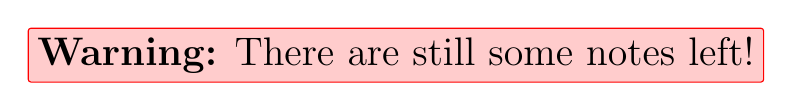
\begin{tikzpicture}[baseline=(A.south)]
    \node (A) [] at (0,0){};
    \node [rounded corners=1pt,rectangle, draw=red, fill=red!20,text=black](B) at (0.1ex,0ex){
        \Large \raggedright {\bf Warning:} There are still some notes left!
    };
 \end{tikzpicture}
\end{center}
 \vspace{1ex}
\fi
}
\makeatletter
\def\myaddcontentsline#1#2#3{%
  \addtocontents{#1}{\protect\contentsline{#2}{#3}{Section \thesubsection\ at p. \thepage}{}}}

\ifWorkInProgress
\renewcommand{\@todonotes@addElementToListOfTodos}{%
    \if@todonotes@colorinlistoftodos%
        \myaddcontentsline{tdo}{todo}{{%
            \colorbox{\@todonotes@currentbackgroundcolor}%
                {\textcolor{\@todonotes@currentbackgroundcolor}{o}}%
            \ \@todonotes@caption}}%
    \else%
        \myaddcontentsline{tdo}{todo}{{\@todonotes@caption}}%
   \fi}%
\newcommand*\mylistoftodos{%
  \begingroup
       \setbox\@tempboxa\hbox{Section 9.9 at p. 99}%
       \renewcommand*\@tocrmarg{\the\wd\@tempboxa}%
       \renewcommand*\@pnumwidth{\the\wd\@tempboxa}%
       \listoftodos%
  \endgroup
}
\fi
\makeatother
\definecolor{lightgreen}{rgb}{0.86, 0.93, 0.78}
\definecolor{bordergreen}{rgb}{0.55, 0.76, 0.74}
\definecolor{lightblue}{rgb}{0.70, 0.90, 0.99}
\definecolor{borderblue}{rgb}{0.01, 0.66, 0.96}
\definecolor{lightamber}{rgb}{1, 0.93, 0.70}
\definecolor{borderamber}{rgb}{1, 0.76, 0.03}
\definecolor{lightcolor4}{rgb}{ 0.93, 0.70, 1}
\definecolor{bordercolor4}{rgb}{0.76, 0.03, 1}
\definecolor{lightcolor5}{rgb}{0.78,0.86,0.93}
\definecolor{bordercolor5}{rgb}{0.74,0.55,0.76}
\newcommand{\dnote}[1]{\stepcounter{notecount}\todo[inline,bordercolor=bordergreen,linecolor=bordergreen,color=lightgreen]{\footnotesize{\sc \bf Dominik:} #1}{}}
\newcommand{\dsnote}[1]{\stepcounter{notecount}\todo[bordercolor=bordergreen,linecolor=bordergreen,color=lightgreen, fancyline]{\footnotesize{\sc \bf Dominik:} #1}{}}
\newcommand{\jnote}[1]{\stepcounter{notecount}\todo[inline,bordercolor=borderblue,linecolor=borderblue,color=lightblue]{\footnotesize{\sc \bf Jo\"el:} #1}{}}
\newcommand{\jsnote}[1]{\stepcounter{notecount}\todo[bordercolor=borderblue,linecolor=borderblue,color=lightblue, fancyline]{\footnotesize{\sc \bf Jo\"el:} #1}{}}
\newcommand{\mnote}[1]{\stepcounter{notecount}\todo[inline,bordercolor=borderamber,linecolor=borderamber,color=lightamber]{\footnotesize{\sc \bf Marta:} #1}{}}
\newcommand{\msnote}[1]{\stepcounter{notecount}\todo[bordercolor=borderamber,linecolor=borderamber,color=lightamber,
 fancyline]{{\scriptsize\sc \bf Marta:} #1}{}}
\newcommand{\enote}[1]{\stepcounter{notecount}\todo[inline,bordercolor=bordercolor4,linecolor=bordercolor4,color=lightcolor4]{\footnotesize{\sc \bf Eike:} #1}{}}
\newcommand{\esnote}[1]{\stepcounter{notecount}\todo[bordercolor=bordercolor4,linecolor=bordercolor4,color=lightcolor4, fancyline]{\footnotesize{\sc \bf Eike:} #1}{}}
\newcommand{\tnote}[1]{\stepcounter{notecount}\todo[caption={},inline,bordercolor=bordercolor5,linecolor=bordercolor5,color=lightcolor5]{\footnotesize{\sc \bf Tal:} #1}{}}
\newcommand{\tsnote}[1]{\stepcounter{notecount}\todo[caption={},bordercolor=bordercolor5,linecolor=bordercolor5,color=lightcolor5, fancyline]{\footnotesize{\sc \bf Tal:} #1}{}}

%----- Algorithm Environment ----------------------------------
\RequirePackage[noend]{sty/algpseudocodex}
%Header for Algorithms/Functionalities
\newcommand{\algoHead}[1]{\vspace{0.2em} \underline{\textbf{#1}} \vspace{0.3em}}
\newcommand{\algoHeadExt}[2]{\vspace{0.2em} \underline{\textbf{#1} #2} \vspace{0.3em}}
%Multiline Algo-States
\makeatletter
\algnewcommand{\ExtendedState}[1]{\State
\parbox[t]{\dimexpr\linewidth-\ALG@thistlm}{\hangindent=\algorithmicindent\strut\hangafter=3#1\strut}}
\makeatother
%Algorithms States
\algnewcommand\algorithmicinput{\textbf{Input:}}
\algnewcommand\Input{\item[\algorithmicinput]}
\renewcommand{\algorithmicensure}{\textbf{Output:}}
\algrenewcommand\algorithmicrequire{\textbf{Input:}}
\algrenewcommand\algorithmicensure{\textbf{Output:}}
%Algo Comments
\definecolor{commentcolor}{HTML}{6698FF}
\algrenewcommand{\algorithmiccomment}[1]{\vspace*{-.3em}{\color{commentcolor}\smash{//} #1}}
%Inline ifs
\algnewcommand{\IIf}[1]{\State\algorithmicif\ #1\ \algorithmicthen}
\algnewcommand{\EndIIf}{\unskip\ \algorithmicend\ \algorithmicif}


%----- Box Environment -----------------------------------------
% v 2019.1.DT small skips
%---
 \RequirePackage{varwidth}
 \RequirePackage{color}
 \RequirePackage[most]{tcolorbox}%with most option


%----- Protocol Boxes
 \newtcolorbox{titlebox}[5]{enhanced,halign=center,colframe=black,colback=white,boxrule={#3},arc={#2},auto outer arc,%
 %breakable,
 pad at break*=5pt,vfill before first,before={\par\smallskip\noindent},after={\par\smallskip},top=12pt,left=0pt,right=2pt,%
 enlarge top by=1pt,%enlarge bottom by=7pt,%
 fontupper=\small,
 title={\rule[-.3\baselineskip]{0pt}{\baselineskip}\sffamily\bfseries\scriptsize #1}, varwidth boxed
 title*=-30pt,
 attach boxed title to top left={yshift=-10pt,xshift=10pt}, coltitle=black,
 boxed title style={colback=white,boxrule={#5},arc={#4},auto outer arc},
 }

 \newtcolorbox{notitlebox}{enhanced,halign=center,colframe=black,colback=white,boxrule={0.5pt},arc={0.5pt},auto outer arc,
  pad at break*=5pt,vfill before first,after={\par\smallskip},left=4pt,
  attach boxed title to top left={yshift=-10pt,xshift=10pt}, coltitle=black
}

 \newenvironment{systembox}[1]
 {\vspace{\baselineskip}\begin{titlebox}{\normalsize Functionality #1}{2.5pt}{1pt}{3.5pt}{1pt}}
 {\end{titlebox}}

 \newenvironment{protocolbox}[1]
 {\begin{titlebox}{Protocol \normalfont #1}{0.5pt}{0.5pt}{1pt}{0.75pt}}
 {\end{titlebox}}

  \newenvironment{simulatorbox}[1]
 {\begin{titlebox}{\normalsize Simulator #1}{0.5pt}{0.5pt}{2pt}{0.75pt}}
 {\end{titlebox}}

  \newenvironment{gamebox}[1]
 {\begin{titlebox}{\normalsize Game #1}{0.5pt}{0.5pt}{2pt}{0.75pt}}
 {\end{titlebox}}

  \newenvironment{processbox}[1]
 {\begin{titlebox}{Process \normalfont #1}{0.5pt}{0.5pt}{1pt}{0.75pt}}
 {\end{titlebox}}

 \newenvironment{algobox}[1]
 {\begin{titlebox}{\normalsize Algorithm #1}{0.5pt}{0.5pt}{1pt}{0.75pt}}
 {\end{titlebox}}

 \newenvironment{funcbox}[1]
 {\begin{titlebox}{Function \normalfont #1}{0.5pt}{0.5pt}{1pt}{0.75pt}}
 {\end{titlebox}}

 \newenvironment{anybox}[1]
 {\begin{titlebox}{ \normalsize #1}{0.5pt}{0.5pt}{1pt}{0.75pt}}
 {\end{titlebox}}

%----- Reference magic ---------------------------------------------------------
%Enable reference of descriptions
\makeatletter
\let\orgdescriptionlabel\descriptionlabel
\renewcommand*{\descriptionlabel}[1]{%
  \let\orglabel\label
  \let\label\@gobble
  \phantomsection
  \edef\@currentlabel{#1}%
  %\edef\@currentlabelname{#1}%
  \let\label\orglabel
  \orgdescriptionlabel{#1}%
}
\makeatother

% Properly reference invariants
\newlist{invariants}{enumerate}{1}
\setlist[invariants,1]{label=\arabic*.,ref=\theinvariantsi}

\makeatletter
\if@cref@capitalise
	\crefname{invariantsi}{Invariant}{Invariants}
\else
	\crefname{invariantsi}{invariant}{invariants}
\fi
\makeatother




%----- Code markers ---------------------------------------------------------

\usepackage[noend]{sty/algpseudocodex}

% Markers
% Usage: turn on line-numbering (\begin{algorithmic}[1]) and then insert
%        \linemarker{foo} right before the line
% (Note this doesn't belong here, but neither does loading algpseudocodex
% which has precede it.)
\makeatletter
\global\def\@linemarker{}
\algrenewcommand{\alglinenumber}[1]{%
	\ifdefempty{\@linemarker}{
		\rule{7pt}{0pt}
	}{
		\rlap{
			\footnotesize\textcolor{red}{\@linemarker}:
			\global\def\@linemarker{}
		}{\rule{7pt}{0pt}}
	}
}
\algnewcommand{\linemarker}[1]{\global\def\@linemarker{#1}}

\newcommand{\refmarker}[1]{line~[\textcolor{red}{#1}]}
\newcommand{\refmarkers}[1]{lines~[\textcolor{red}{#1}]}

\newcounter{markercounter}
\newcommand\newmarker[1]{
	\stepcounter{markercounter}
	\csedef{#1}{\alph{markercounter}}
}
\makeatother

%%% Local Variables:
%%% mode: latex
%%% TeX-master: "../main"
%%% End:

% !TEX root = ../main.tex
%
%  ADD NEW NOTATION at the bottom
%
%-------------------------------------------------------------------------------
%  Font and Notation
%-------------------------------------------------------------------------------
\newcommand{\xmath}[1]{\ensuremath{#1}\xspace}

\newcommand{\N}{\ensuremath{\mathds{N}}\xspace}
% \newcommand{\R}{\ensuremath{\mathbbm{R}}\xspace}
\newcommand{\Q}{\ensuremath{\mathds{Q}}\xspace}
\newcommand{\Z}[0]{\ensuremath{\mathds{Z}}\xspace}
\newcommand{\Zp}[0]{\ensuremath{\Z_p}\xspace}
\newcommand{\powerset}[1]{\ensuremath{\mathcal{P}(#1)}\xspace}

\newcommand{\iseq}[0]{\ensuremath{\overset{?}{=}}}
%-------------------------------------------------------------------------------
%  Fonts used in this project
%-------------------------------------------------------------------------------
\newcommand{\command}[1]{\xmath{\textsc{#1}}}
\newcommand{\algorithm}[1]{\xmath{\textsf{#1}}}
\newcommand{\variable}[1]{\xmath{\textnormal{\textsf{#1}}}}
\newcommand{\parameter}[1]{\xmath{\texttt{#1}}}
\newcommand{\keyword}[1]{\xmath{{\normalfont\texttt{#1}}}}

\newcommand{\hardprobfont}[1]{\texorpdfstring{\ensuremath{\textsf{#1}}}{#1}}
\newcommand{\gamefont}[1]{\texorpdfstring{{\normalfont \ensuremath{\textsf{#1}}}}{#1}}
\newcommand{\algorithmfont}[1]{\texorpdfstring{\algorithm{#1}}{#1}}

\newcommand{\bigO}{\ensuremath{\textsf{O}}\xspace}

% assumptions
\newcommand{\sdh}[0]{\textnormal{\hardprobfont{DSSDH}}\xspace}

% Security notions
\newcommand{\indcca}[0]{\gamefont{IND-CCA}\xspace}
\newcommand{\indrcca}[0]{\gamefont{IND-RCCA}\xspace}
\newcommand{\indcpa}[0]{\gamefont{IND-CPA}\xspace}
\newcommand{\mmindcca}[0]{\gamefont{mmIND-CCA}\xspace}
\newcommand{\mmindrcca}[0]{\gamefont{mmIND-RCCA}\xspace}
\newcommand{\mmowrcca}{\gamefont{mmOW-RCCA}\xspace}
%\newcommand{\wmmindcca}[0]{\gamefont{w-mmIND-CCA}\xspace}
%\newcommand{\sceo}{\gamefont{S-CEO}\xspace}
%\newcommand{\msceo}{\gamefont{MS-CEO}\xspace}
%\newcommand{\ssceo}{\gamefont{MS-sCEO}\xspace}
\newcommand{\ufcma}[0]{\gamefont{EUF-CMA}\xspace}
%\newcommand{\rsufcma}[0]{\gamefont{RS-EUF-CMA}\xspace}
%\newcommand{\ersufcma}[0]{\gamefont{EUF-RCMA}\xspace}
%\newcommand{\ahrsufcma}[0]{\gamefont{A}\ersufcma}
%\newcommand{\shrsufcma}[0]{\gamefont{S}\ersufcma}
\newcommand{\mmufcma}[0]{\gamefont{mmEUF-CMA}\xspace}

\newcommand{\op}[0]{\gamefont{OP}\xspace}

\newcommand{\kc}[0]{\gamefont{KC}\xspace}
\newcommand{\rkc}[0]{\gamefont{RKC}\xspace}

%-------------------------------------------------------------------------------
%  General notation
%-------------------------------------------------------------------------------
%Fields, sets, tions
\newcommand{\aset}[1]{\left\{ { #1 }\right\}}% {#1}
\newcommand{\union}{\ensuremath{\cup}}
\DeclarePairedDelimiter\abs{\lvert}{\rvert}% |#1|
%\newcommand{\nicevec}[1]{\overrightarrow{#1}}
\newcommand{\Mspace}{\ensuremath{\mathcal{M}}\xspace}


%Distribution
\newcommand{\getsDist}{\twoheadleftarrow} %<<--

%Player sets, adversary
\newcommand{\party}{P\xspace}
\newcommand{\PS}{\mathcal{P}}
\newcommand{\HS}{\mathcal{H}} %honest parties
\newcommand{\CS}{\mathcal{Z}} %corrupted parties
\newcommand{\crashedP}{\mathcal{C}}
\newcommand{\passiveP}{\mathcal{Z}^p}
\newcommand{\semiP}{\mathcal{Z}^s}
\newcommand{\failstopP}{\mathcal{Z}^f}
\newcommand{\Adv}[1][\relax]{\xmath{\mathcal{A}_{#1}}}
\newcommand{\Bdv}[1][\relax]{\xmath{\mathcal{B}_{#1}}}


%Graph and neighborhood
\newcommand{\graph}{G}
\newcommand{\graphfam}{\mathcal{G}}% G
\newcommand{\nbh}[1]{\mathbf{N}_G(#1)}% N(v)
\newcommand{\nbhi}[2]{\mathbf{N}_{G_{#1}}(#2)}
\newcommand{\nbhc}[1]{\mathbf{N}_G[#1]}% N[v]

% oracles
\newcommand{\oracleDec}[0]{\ensuremath{\mathcal{O}_{\text{\mmpkeDec}}(\cdot,\mmpkesk,\cdot)}\xspace}


%-------------------------------------------------------------------------------
% Global parameters
%-------------------------------------------------------------------------------
%Security param
\newcommand{\secparam}{\xmath{\kappa}}
\newcommand{\negl}{\text{negl}}
\newcommand{\poly}{\mathsf{poly}}

%-------------------------------------------------------------------------------
%  UC and Functionalites
%-------------------------------------------------------------------------------
\newcommand{\ucexe}[3]{\command{EXEC}_{#1,#2,#3}}
%\newcommand{\uchyb}[2]{\command{HYB}_{#1,#2}}
\newcommand{\uchyb}[1]{\mathcal{H}_{#1}}
\newcommand{\ucenv}{\xmath{\mathcal{Z}}}
\newcommand{\ucsim}[1][\relax]{\xmath{\mathcal{S}_{\textsc{#1}}}}
\newcommand{\indist}[1][\relax]{\ensuremath{\overset {#1}{\approx}}}

%Turning machines
\newcommand{\itm}{\xmath{\mathtt{ITM}}}
\newcommand{\iti}{\xmath{\mathtt{ITI}}}

%Protocol
\newcommand{\prot}{\Pi}

%Functionalities
\newcommand{\Func}[1][\relax]{\xmath{\mathcal{F}_{\normalfont\textsc{#1}}}}
\newcommand{\GFunc}[1][\relax]{\xmath{\mathcal{G}_{\normalfont\textsc{#1}}}}
%\newcommand{\wrapper}{\mathcal{W}}

%M/S-ID
\newcommand{\sid}{\mathsf{sid}}
\newcommand{\pid}{\mathsf{pid}}

%------------------------------
%  ADD NEW NOTATION below
%-------------------------------

\newcommand{\true}{\keyword{true}}
\newcommand{\false}{\keyword{false}}

% === Misc ===

\newcommand{\getsr}{\gets_{\scriptscriptstyle\$}} %dollar behind arrow
\renewcommand{\getsr}{\mathrel{\vbox{\offinterlineskip\ialign{
        \hfil##\hfil\cr
        \hspace{0.1em}$\scriptscriptstyle\$$\cr
        $\leftarrow$\cr
      }}}} %dollar on arrow
\newcommand{\getsl}{\rightarrow_{\scriptscriptstyle\$}} %dollar behind arrow
\renewcommand{\getsl}{\mathrel{\vbox{\offinterlineskip\ialign{
        \hfil##\hfil\cr
        \hspace{-0.2em}$\scriptscriptstyle\$$\cr
        $\rightarrow$\cr
      }}}} %dollar on arrow

\newcommand{\bits}{\{0,1\}}
\newcommand{\wc}{*}

%%% General formating
\newcommand{\mdef}[1]{{\ensuremath{#1}}\xspace}      % Math Def which can also be used in normal text.
\newcommand{\term}[1]{\mdef{\mathsf{#1}}}            % Math Term/Algorithm
\newcommand{\method}[1]{\mdef{\textnormal{\tt*#1}}}  % Method in a class
%\newcommand{\str}[1]{\mdef{\texttt{"#1"}}}           % Constant
\newcommand{\attrib}[1]{\mdef{\mathsf{#1}}}          % Attribute in a class
\newcommand{\myvar}[1]{\mdef{#1}}                    % Concrete variable. I.e. an instantiated object.
\newcommand{\func}[1]{\mdef{\mathsf{#1}}}            % Stand alone function / algorithm.
\newcommand{\myvec}[1]{\vec{#1}}
\newcommand{\literal}[1]{\mdef{\text{\normalfont \it`#1'}}}			% String literals

\newcommand{\md}{\textrm{-}}
\newcommand{\algoskip}{\smallskip}

\newcommand{\set}[1]{\{#1\}}

\newcommand{\ititle}[1]{{\bf #1}}
\newcommand{\from}{\gets}



% ==========================
% === CGKA Functionality ===
% ==========================


% === History Graph ===

\newcommand{\hg}{\term{HG}}
\newcommand{\hge}{V}

%\newcommand{\hgroot}{\hge_{\mathsf{root}}}
\newcommand{\hgroot}[1]{\mathsf{root}_{#1}}
\newcommand{\rootCount}{\mathsf{rootCtr}}
\newcommand{\numRoot}{rt}

\newcommand{\hgl}{\literal{lbl}}
\newcommand{\hgt}{\literal{type}}
\newcommand{\hgli}{\literal{init}}
\newcommand{\hgla}{\literal{add}}
\newcommand{\hglr}{\literal{rem}}
\newcommand{\hglu}{\literal{up}}

\newcommand{\hgm}{\mathsf{mem}}
\newcommand{\hgk}{\mathsf{key}}
\newcommand{\hgc}{\mathsf{chall}}
\newcommand{\hgpar}{\mathsf{par}}
\newcommand{\hgexp}{\mathsf{exp}}

\newcommand{\ptr}{\textsf{CurEp}}
\newcommand{\hgnew}{\method{new-ep}}
\newcommand{\ep}{E}

\newcommand{\grp}{G}

\newcommand{\hgorig}{\mathsf{sndr}}
\newcommand{\hgact}{\mathsf{act}}
\newcommand{\hginj}{\textsf{inj}}
\newcommand{\setvert}{\mathsf{HG}}
\newcommand{\pgod}{\id_\mathsf{creator}}

\newcommand{\msgS}{C}
\newcommand{\msgR}{c}
\newcommand{\hgnodeid}{{\normalfont\textsf{epid}}}
\newcommand{\hgnctr}{\textsf{epCtr}}

\newcommand{\hgConsistent}{\method{HG-is-consistent}}
\newcommand{\authPreserved}{\method{auth-is-preserved}}
\newcommand{\members}{\method{mem}}

% === Keywords ===
\newcommand{\KwReq}{\textbf{req}}
\newcommand{\KwTry}{\textbf{try}}
\newcommand{\KwWin}{\textbf{win}}
\newcommand{\KwPub}{\textbf{pub}}
\newcommand{\KwSafe}{\textbf{safe}}
\newcommand{\KwConf}{\textnormal{\textbf{confidential}}}
\newcommand{\KwAuth}{\textnormal{\textbf{authentic}}}
\newcommand{\KwCanInj}{\textbf{inj-allowed}}
\newcommand{\KwAss}{\textbf{assert}}
\newcommand{\KwRestrEnv}{\textbf{restrict}}
\newcommand{\KwParse}{\textbf{parse}}

% === Safe ===
\newcommand{\ancestor}{\text{\sffamily *ancestor}}
\newcommand{\safeDetached}{\text{\sffamily\bfseries *in-detached-tree}}

% === PKI ===
\newcommand{\SSK}{\term{SSK}}
\newcommand{\kbpk}{\term{kp}}
\newcommand{\kbsk}{\term{sk}}
\newcommand{\KBSK}{\term{SK}}
\newcommand{\KBSPK}{\term{SPK}}
\newcommand{\corrSPK}{\term{Exposed}}
\newcommand{\regSPK}{\term{Registered}}
%\newcommand{\honPK}{\term{HonestPK}}


%\newcommand{\pkig}{\mathsf{get\md{}pk}}
\newcommand{\getKbSks}{get\md{}sks}

\newcommand{\pkepk}{\mathsf{pk}}
\newcommand{\pkesk}{\mathsf{sk}}



% === Safe ===
\newcommand{\safeKnow}{\text{\sffamily\bfseries *know}}
\newcommand{\safeStateKnown}{\text{\sffamily\bfseries *exposed}}
\newcommand{\safeHeals}{\text{\sffamily\bfseries *heals}}
\newcommand{\safeInjAct}{\text{\sffamily\bfseries *secrets-injected}}
\newcommand{\safeCanTraverse}{\text{\sffamily\bfseries *can-traverse}}
\newcommand{\safeExpWelcome}{\text{\sffamily\bfseries *leaf-welcome-key-reuse}}
\newcommand{\safeDetachedTree}{\method{in-det-tree}}
\newcommand{\safePartySecPres}{\method{party-secrecy-is-preserved}}
\newcommand{\safePartyExp}{\method{party-secs-are-exposed}}
\newcommand{\safeRestoresPartySec}{\method{restores-party-secrecy}}


% === Functionalities ===
\newcommand{\funcCGKA}{\Func[cgka]}
%\newcommand{\funcPKI}{\GFunc[as]}					% authentication service
%\newcommand{\funcKB}{\GFunc[ks]}					% key service
\newcommand{\funcPKI}{\Func[aks]}					% authentication service
\newcommand{\funcKB}{\Func[ks]}					% key service

\newcommand{\funcPKIideal}{\Func[as]^{\normalfont\textsc{iw}}}
\newcommand{\funcKBideal}{\Func[ks]^{\normalfont\textsc{iw}}}

% ==================
% === mmGSD-RCCA ===
% ==================

\newcommand{\vrxCtr}{N}
\newcommand{\vrxNum}{u}
\newcommand{\vrxNumT}{v}
\newcommand{\vrxSeed}[1]{\term{Seed}[#1]}
\newcommand{\vrxUsed}{\term{Used}}
\newcommand{\Edges}{\term{Dependencies}}
\newcommand{\decrypted}{\term{Decrypted}}
\newcommand{\vrxCorr}{\term{Corr}}
\newcommand{\funcPK}{\method{pk}}
\newcommand{\hashlbl}{\term{lbl}}
\newcommand{\vrx}[1]{u_{\textsf{#1}}}


% ==================
% === Primitives ===
% ==================

% === Groups ===
% \newcommand{\G}{\ensuremath{\mathds{G}}\xspace}
\newcommand{\Grp}{\ensuremath{\mathds{G}}\xspace}
\newcommand{\Group}{\ensuremath{\mathcal{G}}\xspace}
\newcommand{\GGen}{\term{GGen}\xspace}

% === Nominal Groups ===
\newcommand{\ngroup}{\ensuremath{\mathcal{N}}\xspace}
\newcommand{\nG}{\ensuremath{\mathcal{G}}\xspace}
\newcommand{\nGE}{\ensuremath{\mathcal{E}_H}\xspace}
\newcommand{\nGU}{\ensuremath{\mathcal{E}_U}\xspace}
\newcommand{\nGexp}{\textnormal{\sf exp}\xspace}

% === Accumulator ===
\newcommand{\acc}[0]{\term{Acc}}
\newcommand{\wacc}[0]{\term{wAcc}}

\newcommand{\accSetup}[0]{\term{Setup}}
\newcommand{\accEval}[0]{\term{Eval}}
\newcommand{\accProve}[0]{\term{Prove}}
\newcommand{\accVrfy}[0]{\term{Vrfy}}

\newcommand{\waccSetup}[0]{\term{wSetup}}
\newcommand{\waccEval}[0]{\term{wEval}}
\newcommand{\waccProve}[0]{\term{wProve}}
\newcommand{\waccVrfy}[0]{\term{wVrfy}}

\newcommand{\accpub}[0]{\ensuremath{pp}\xspace}
\newcommand{\acctrap}[0]{\ensuremath{\tau}\xspace}
\newcommand{\accSpace}[0]{\ensuremath{\mathcal{X}}\xspace}
\newcommand{\accValue}[0]{\ensuremath{\mathit{acc}}\xspace}
\newcommand{\accaux}[0]{\ensuremath{\mathit{aux}}\xspace}
\newcommand{\accProof}[0]{\ensuremath{\pi}\xspace}

% === mmPKE and mmAPKE===
\newcommand{\mmPKE}[0]{\term{mmPKE}}

\newcommand{\mmpkeKeyGen}[0]{\term{KG}}
\newcommand{\mmpkeEnc}[0]{\term{Enc}}
\newcommand{\mmpkeDec}[0]{\term{Dec}}
\newcommand{\mmpkeExt}[0]{\term{Ext}}

\newcommand{\mmpkeKeyGenL}[0]{\mmPKE.\term{KG}\xspace}
\newcommand{\mmpkeEncL}[0]{\mmPKE.\term{Enc}\xspace}
\newcommand{\mmpkeDecL}[0]{\mmPKE.\term{Dec}\xspace}
\newcommand{\mmpkeExtL}[0]{\mmPKE.\term{Ext}\xspace}

\newcommand{\mmpkesk}{\term{dk}}
\newcommand{\mmpkepk}{\term{ek}}
\newcommand{\mmpkessk}{\term{ssk}}
\newcommand{\mmpkespk}{\term{spk}}
\newcommand{\mmpkersk}{\term{rsk}}
\newcommand{\mmpkerpk}{\term{rpk}}


\newcommand{\mmpkeskL}{\mmPKE.\term{sk}}
\newcommand{\mmpkepkL}{\mmPKE.\term{pk}}
\newcommand{\mmpkePK}{\ensuremath{\vec{\mathsf{PK}}}\xspace}
\newcommand{\mmpkeSPK}{\ensuremath{\vec{\mathsf{SPK}}}\xspace}

\newcommand{\mmpkeCtxt}{\ensuremath{{\mmPKE}\term{Ctxt}}\xspace}

\newcommand{\leak}[0]{\term{leak}}
% === mKEM ===
\newcommand{\mKEM}[0]{\term{mKEM}}

\newcommand{\mKEMSetup}[0]{\term{mSetup}}
\newcommand{\mKEMGen}[0]{\term{mKeyGen}}
\newcommand{\mKEMEncaps}[0]{\term{mEncaps}}
\newcommand{\mKEMDecaps}[0]{\term{mDecaps}}
\newcommand{\mKEMExt}[0]{\term{mExt}}

\newcommand{\mKEMpub}[0]{\term{pp}}
\newcommand{\mKEMsk}[0]{\term{sk}}
\newcommand{\mKEMpk}[0]{\term{pk}}

\newcommand{\mKEMpubL}[0]{\mKEM.\term{pp}}
\newcommand{\mKEMskL}[0]{\mKEM.\term{sk}}
\newcommand{\mKEMpkL}[0]{\mKEM.\term{pk}}

% === mPKE ===
\newcommand{\mPKE}[0]{\term{mPKE}}

\newcommand{\mPKESetup}[0]{\term{mSetup}}
\newcommand{\mPKEGen}[0]{\term{mGen}}
\newcommand{\mPKEEnc}[0]{\term{mEnc}}
\newcommand{\mPKEDec}[0]{\term{mDec}}
\newcommand{\mPKEExt}[0]{\term{mExt}}

\newcommand{\mPKEpub}[0]{\term{pp}}
\newcommand{\mPKEsk}[0]{\term{sk}}
\newcommand{\mPKEpk}[0]{\term{pk}}

\newcommand{\mPKEpubL}[0]{\mPKE.\term{pp}}
\newcommand{\mPKEskL}[0]{\mPKE.\term{sk}}
\newcommand{\mPKEpkL}[0]{\mPKE.\term{pk}}

\newcommand{\mPKEKS}{\mathcal{PK}}

% === Redactable Signatures ===
\newcommand{\rs}{\term{RS}}
\newcommand{\rssign}{\term{Sign}}
\newcommand{\rskeygen}{\term{KeyGen}}
\newcommand{\rsvrfy}{\term{Vrfy}}
\newcommand{\rsred}{\term{Reduce}}

\newcommand{\rssignL}{\rs.\term{Sign}}
\newcommand{\rskeygenL}{\rs.\term{KeyGen}}
\newcommand{\rsvrfyL}{\rs.\term{Vrfy}}
\newcommand{\rsredL}{\rs.\term{Redact}}

\newcommand{\rssk}{\term{sk}}
\newcommand{\rsvk}{\term{vk}}

\newcommand{\rsskL}{\rs.\term{sk}}
\newcommand{\rsvkL}{\rs.\term{vk}}

\newcommand{\rdclass}{\term{RPC}}
\newcommand{\rdclassset}{\term{RPCS}}
\newcommand{\rd}{\term{rp}}

\newcommand{\rdclassBGM}{\ensuremath{\rdclass^{\textnormal{SAIK}}}\xspace}
\newcommand{\rdclasssetBGM}{\ensuremath{\rdclassset^{\textnormal{SAIK}}}\xspace}
% === Enhanced Red. Signatures ===
\newcommand{\ers}{\term{HRS}}
\newcommand{\erssign}{\term{Sign}}
\newcommand{\erskeygen}{\term{KeyGen}}
\newcommand{\ersvrfy}{\term{Vrfy}}
\newcommand{\ersred}{\term{Reduce}}

\newcommand{\erssignL}{\ers.\term{Sign}}
\newcommand{\erskeygenL}{\ers.\term{KeyGen}}
\newcommand{\ersvrfyL}{\ers.\term{Vrfy}}
\newcommand{\ersredL}{\ers.\term{Redact}}

\newcommand{\erssk}{\term{sk}}
\newcommand{\ersvk}{\term{vk}}

\newcommand{\ersskL}{\ers.\term{sk}}
\newcommand{\ersvkL}{\ers.\term{vk}}

% === PK Encryption ===
\newcommand{\pke}{\term{PKE}}                       % PK Encryption Scheme
\newcommand{\pkkg}{\pke.\term{kg}}                  % PK Key Gen
\newcommand{\pkenc}{\pke.\term{enc}}                % PK Encrypt
\newcommand{\pkdec}{\pke.\term{dec}}                % PK Decrypt
\newcommand{\pkpk}{\term{ek}}                      % PK Enc public key
\newcommand{\pksk}{\term{dk}}                      % PK Enc secret key
\newcommand{\pkpkL}{\pke.\term{ek}}                      % PK Enc public key
\newcommand{\pkskL}{\pke.\term{dk}}                      % PK Enc secret key


% === Signing scheme ===
\newcommand{\sigscheme}{\term{Sig}}
\newcommand{\sigsign}{\sigscheme.\term{sign}}
\newcommand{\sigvrf}{\sigscheme.\term{vrf}}
\newcommand{\sigkg}{\sigscheme.\term{KG}}
\newcommand{\sig}{\term{sig}}
\newcommand{\spk}{\term{spk}}
\newcommand{\ssk}{\term{ssk}}

% === DEM scheme ===
\newcommand{\dem}{\term{DEM}}
\newcommand{\demKeyset}{\ensuremath{\mathcal{K}}}
\newcommand{\demEnc}{\term{D}}
\newcommand{\demDec}{\ensuremath{\term{D}^{-1}}}

% === MAC scheme ===
\newcommand{\mac}{\term{MAC}}
\newcommand{\mackeyspace}{\ensuremath{\mathcal{K}}\xspace}
\newcommand{\mactag}{\mac.\term{tag}}
\newcommand{\macvrf}{\mac.\term{vrf}}
\newcommand{\mtag}{\term{tag}}


% === KDF ===
\newcommand{\kdf}{\term{KDF}}
\newcommand{\hkdf}{\term{HKDF}}
\newcommand{\hkdfexp}{\hkdf.\term{Exp}}
\newcommand{\hkdfext}{\hkdf.\term{Ext}}


% === Hash function ===
\newcommand{\hash}{\term{Hash}}
\newcommand{\CR}{\gamefont{CR}\xspace}

% =======================
% === Data Structures ===
% =======================


% ==== Sets ====
\let\oldemptyset\emptyset                           %Nice empty set
\let\emptyset\varnothing

\newcommand{\setadd}{\ \texttt{+$\gets$}\ }
\newcommand{\setrem}{\ \texttt{-$\gets$}\ }


% === Lists ===
\newcommand{\emptylist}{()}
\newcommand{\append}{\mathrel{+\!\!+}}              % Append an element to a list
\newcommand{\listapp}{\ \texttt{+\!\!+$\gets$}\ }
\newcommand{\reverse}{\term{reverse}}               % Reverses the list
\newcommand{\indexof}{\term{indexof}}
\newcommand{\zip}{\term{zip}}


% === Paths ===
\newcommand{\newpath}{\term{  path}}                % Declare a new path object
\newcommand{\source}{\term{source}}                 % Returns first (deepest) node in a path
\newcommand{\sink}{\term{sink}}                     % Returns last (shallowest) node in a path
\newcommand{\traverses}{\term{traverses}}           % Boolean indicating if path traverses argument node
\newcommand{\meets}{\term{meets}}                   % Returns true iff the 2 argument paths meet
\newcommand{\meetsat}{\term{meetsAt}}               % Returns first (deepest)
%node on both argument paths


%% === Queus & Maps (Legacy) ===
%\newcommand{\enq}{\term{enq}}                       % Enqueu an item into a queue
%\newcommand{\deq}{\term{deq}}                       % Dequeu an item from a queue
%\newcommand{\delete}{\term{del}}                    % Delete an item from a queue
%\newcommand{\clear}{\term{clear}}                   % Delete all entries from an associative array

\newcommand{\gsdLbl}{\term{lbl}}
\newcommand{\adv}[2]{\ensuremath{\textnormal{Adv}_{#2}^{#1}}\xspace}
\newcommand{\advantage}[3]{\textnormal{Adv}_{#2, \text{#3}}^{#1}}			%
\newcommand{\experiment}[2]{\textnormal{Exp}_{#2}^{#1}}			%
\newcommand{\Exp}{\textnormal{Exp}}
\newcommand{\grpSecret}{\textsf{`epoch'}}
\newcommand{\dist}{\mathcal{D}}

\newcommand{\nodeUsed}{\textbf{gen-key-if-nec}}
\newcommand{\reachable}{\textbf{gsd-exp}}

\newcommand{\nUsers}{N}
\newcommand{\nMsgs}{\ell}
\newcommand{\nRcvrs}{n}
\newcommand{\idxUser}{i}
\newcommand{\idxMsg}{j}
\newcommand{\idxRcvr}{k}

\newcommand{\trivialComput}{\method{triv-comput}}
\newcommand{\triggerE}{\variable{ItriggerE}}
\newcommand{\oracle}[1]{\textnormal{\textsf{\bfseries #1}}}

\newcommand{\injects}{\variable{Forges}}
\newcommand{\injected}{\variable{injected}}
\newcommand{\wins}{\variable{Wins}}
\newcommand{\injectsA}{\variable{ForgesAsym}}
\newcommand{\injectsB}{\variable{ForgesSym}}
\newcommand{\injectsBstat}{\variable{ForgesSym'}}
\newcommand{\gforge}{G^\mathsc{forge}}

\newcommand{\dhmmpke}{\term{DH\md mmPKE}}
\newcommand{\huffmanacc}{\term{Huf\md wAcc}}
\newcommand{\huffman}{\algorithm{huffman}}
\newcommand{\bgmHrs}{\normalfont{\algorithm{BGM-HRS}}}
% === Acronyms ===
\DeclareAcronym{hrs}{%
  short=RS, long=Reducible Signature
}
\newcommand{\smashedComment}[1]{\smash{\Comment{#1}}}
\newcommand{\safeExposedSecrets}{\method{exposed-ind-secs}}
\newcommand{\safeExposedGrpSecrets}{\method{exposed-grp-secs}}
\newcommand{\safeSharesSecrets}{\method{share-ind-secs}}
\newcommand{\safeKnowsSecrets}{\method{ind-secs-bad}}
\newcommand{\safeWeakAdd}{\method{exposed-ind-secs-weak}}

\newcommand{\safeGrpSecsSecure}{\method{grp-secs-secure}}
\newcommand{\safeRestoresGrpSec}{\method{all-ind-secs-secure}}
\newcommand{\safeIndSecsSecure}{\method{ind-secs-secure}}

%%% Local Variables:
%%% mode: latex
%%% TeX-master: "../main"
%%% End:

%
%
%%     Macros for Defining the MLS construction
%
%

%%% General formating (already included in macros.tex)
\newcommand{\superscript}[1]{\ensuremath{^{\mbox{\tiny{\textit{#1}}}}}\xspace}
\newcommand{\inc}{\texttt{++}}
% \newcommand{\abs}[1]{\mdef{\left|#1\right|}}        % Absolute value

%%% Counting things
\def \th {\superscript{th}}                         % 'The i-th entry it a list...' --> i\th
\def \st {\superscript{st}}                         % 'The 1-st entry it a list...' --> 1\st
\def \nd {\superscript{nd}}                         % 'The 2-nd entry it a list...' --> 2\nd
%\def \rd {\superscript{rd}}                         % 'The 3-rd entry it a list...' --> 3\rd
\def \etal{{\it et~al.}}

%%% Common sets and variables
\newcommand{\eps}{\mdef{\epsilon}}                  % Empty string


\def \treekemA {TreeKEMv2\xspace}
\def \treekemB {TreeKEMv3\xspace}
%\def \mls {MLSv9\xspace}
\def \mlsfrozen {MLSv9\xspace}
\def \mls {MLS\xspace}
\def \saik {{\normalfont\textsf{SAIK}}\xspace}
\newcommand{\heading}[1]{{\vspace{1ex}\noindent\sc\underline{\smash{#1}}}}
\newcommand{\headingB}[1]{{\vspace{1ex}\noindent\bf{\smash{#1}}}}



% =============
% === Trees ===
% =============

% LBBT definition
\newcommand{\FT}{\term{FT}}                         % Full binary tree
\newcommand{\LBBT}{\term{LBBT}}                     % Left-balanced binary tree
\newcommand{\maxp}{\term{mp2}}                      % Maimum power of 2 smaller than or equal to argument.
\newcommand{\addleaf}{\term{addLeaf}}               % Add a leaf to LBBT_n to get LBBT_n+1
\newcommand{\ltree}{\tree_{\mathsf L}}              % Arbitrary left sub-tree
\newcommand{\rtree}{\tree_{\mathsf R}}              % Arbitrary right sub-tree
\newcommand{\treeArity}{q}
\newcommand{\lbt}[2]{\term{LBT}_{#1,#2}}
\newcommand{\mpow}{\term{max\md pow}}
\newcommand{\leaf}{\term{leaf}}


% Basic stuff
\newcommand{\tree}{\tau}                            % Arbitrary tree
\newcommand{\rt}{\term{root}}                       % Root of a tree
\newcommand{\nodes}{\term{nodes}}                   % The set of nodes in the LT.
\newcommand{\isroot}{\term{isroot}}                 % Returns true iff node is the root.
\newcommand{\isleaf}{\term{isleaf}}                 % Returns true iff node is the root.
\newcommand{\parent}{\term{parent}}                 % Parent of a node
\newcommand{\nodeIndex}{\term{nodeIdx}}				% The node index of a node
\newcommand{\depth}{\term{depth}}
\newcommand{\children}{\term{children}}


% Node labels (unless otherwise defined)
\newcommand{\unmergedLeaves}{\term{unmLvs}} % The set of unmerged leaves


% Tree helper function
\newcommand{\clone}{\term{clone}}					% Returns a deep copy of the tree
\newcommand{\public}{\term{public}}                 % Returns the same LT but with private labels cleared.
\newcommand{\roster}{\term{roster}}                 % Returns the set of group members' IDs.
\newcommand{\leaves}{\term{leaves}}                 % Associative array leafIndex -> leaf.
\newcommand{\leafof}{\term{leafof}}                 % Returns leaf of input ID.
\newcommand{\getleaf}{\term{getLeaf}}               % Finds first blank leaf. If none insert new leaft and return it.
\newcommand{\directpath}{\term{directPath}}		    % Returns the direct path starting at argument leafIndex
\newcommand{\lca}{\term{lca}}                       % Least common ancestor function of two input nodes
\newcommand{\blankpath}{\term{blankPath}}		    % Blanks the direct path starting at argument leafIndex
\newcommand{\mergeleaves}{\term{mergeLvs}}       % Empties the unmergedLeaves set on the direct path
\newcommand{\unmergeleaf}{\term{unmerge}}       % Adds the leaf to the unmergedLeaves set on the direct path


% Node helper functions
\newcommand{\inuse}{\term{inuse}}                   % Returns true iff node has labels
\newcommand{\blank}{\term{blank}} 					% Blanks the node
\newcommand{\resolution}{\term{resolution}}			% Returns the node's resolution (i.e., the set of nodes one needs to encrypt to instead)
\newcommand{\resolvent}{\term{resolvent}}			% Deterimines the resolvent

\newcommand{\id}{\term{id}}                         % An identity



% ========================
% === MLS Construction ===
% ========================

\newcommand{\protCMPKE}{{\normalfont\textsf{CmPKE}}\xspace}
\newcommand{\protMLS}{{\normalfont\textsf{MLS}}}
\newcommand{\protITK}{{\normalfont\textsf{ITK}}\xspace}
\newcommand{\protITKI}{{\normalfont\textsf{ITK-I}}\xspace}
\newcommand{\protITKalt}{{\normalfont\textsf{ITK}\texorpdfstring{\ensuremath{^*}}{*}}\xspace}


% ITK State
\newcommand{\itkSt}{\gamma}
\newcommand{\groupId}{\term{grpId}}
\newcommand{\treeHash}{\term{treeHash}}
\newcommand{\lastAct}{\term{lastAct}}
\newcommand{\applicationSecret}{\term{appSec}}
\newcommand{\membershipKey}{\term{membKey}}
\newcommand{\initSecret}{\term{initSec}}

% State helper functions
\newcommand{\groupContext}{\term{grpCtxt}}



% Construction helper functions
%\newcommand{\applyprops}{
%	\hyperlink{helper:applyprops}{\method{apply-props}}}
\newcommand{\deriveKeys}{{\method{derive-keys}}}
\newcommand{\deriveEpochKeys}{{\method{derive-epoch-keys}}}
\newcommand{\rekeypath}{{\method{rekey-path}}}
\newcommand{\createEpoch}{\method{create-epoch}}
\newcommand{\provState}{\method{create-epoch}}
\newcommand{\nextState}{\method{transition}}
\newcommand{\encSecrets}{\method{encrypt}}
\newcommand{\encSecretsAdd}{\method{encrypt-with-joiner}}
\newcommand{\decSecrets}{\method{decrypt-path-secret}}
\newcommand{\applyact}{\method{apply-act}}
\newcommand{\len}{\texttt{len}}
\newcommand{\signMsg}{\method{authenticate}}
\newcommand{\signMsgAdd}{\method{authenticate-for-joiner}}
\newcommand{\populateSecrets}{\method{get-secrets}}
\newcommand{\setTreeHash}{{\method{set-tree-hash}}}
\newcommand{\computeTreeHash}{{\method{tree-hash}}}


% Construction Variables
\newcommand{\joinerSecret}{\term{joinerSec}}
\newcommand{\epochSecret}{\term{epSec}}
\newcommand{\commitSecret}{\term{commitSec}}
\newcommand{\updatePath}{\term{updPath}}
\newcommand{\updatePathNodes}{\term{updPathNodes}}
\newcommand{\pathSecret}{\term{pathSec}}
\newcommand{\pathSecrets}{\term{pathSecs}}
\newcommand{\encPathSecrets}{\term{encPathSecs}}
\newcommand{\encGroupSecret}{{\normalfont\textit{ctxt}}}
\newcommand{\encGroupSecrets}{\term{encGrpSecs}}
\newcommand{\nodeSecret}{\term{nodeSec}}
\newcommand{\auxData}{\term{auxData}}
\newcommand{\updatedPks}{\term{updEKs}}
\newcommand{\redactedSig}{\sig'}
\newcommand{\redactedUpPks}{\updatedPks'}
\newcommand{\pathSecCtxt}{{\normalfont\textit{Ctxt}}}
\newcommand{\pathSecCtxtInd}{{\normalfont\textit{ctxt}}}
\newcommand{\genPKIkeys}{\method{AKS-kgen}}
\newcommand{\KwQuery}{\keyword{query}}
\newcommand{\epochSecretVec}{\term{EpSecs}}
\newcommand{\fullpath}{\term{path}}
\newcommand{\concat}{\mathrel{+\!\!+}}
\newcommand{\inSubtree}{\term{inSubtree}}
\newcommand{\getPathSecsMap}{\method{rcvrs-of-path-secs}}
\newcommand{\getWeights}{\method{weights}}
\newcommand{\myReduction}{\method{my-reduction-pattern}}
\newcommand{\confTag}{\term{confTag}}
\newcommand{\macsig}{\term{tag}}

% Legacy
\newcommand{\ckagk}{\mdef{I}}                       % CGKA group key

\crefname{appendix}{App.}{Apps.}%
\crefname{section}{Sec.}{Secs.}%

%%\ccsPaper{9999} % TODO: replace with your paper number once obtained

\copyrightyear{2022} 
\acmYear{2022} 
\setcopyright{rightsretained} 
\acmConference[CCS '22]{Proceedings of the 2022 ACM SIGSAC Conference on Computer and Communications Security}{November 7--11, 2022}{Los Angeles, CA, USA}
\acmBooktitle{Proceedings of the 2022 ACM SIGSAC Conference on Computer and Communications Security (CCS '22), November 7--11, 2022, Los Angeles, CA, USA}
\acmDOI{10.1145/3548606.3560632}
\acmISBN{978-1-4503-9450-5/22/11}

\begin{document}
\title{Server-Aided Continuous Group Key Agreement}

\author{Joël Alwen}
\email{alwenjo@amazon.com}
\affiliation{%
	\institution{AWS-Wickr}
	\city{New York}
	\state{NY}
	\country{USA}
}
\author{Dominik Hartmann}
\email{dominik.hartmann@rub.de}
\orcid{0000-0002-0379-7903}
\affiliation{%
	\institution{Ruhr-University Bochum}
	\city{Bochum}
	\country{Germany}
}
\author{Eike Kiltz}
\email{eike.kiltz@rub.de}
\orcid{0000-0003-1178-048X}
\affiliation{%
  \institution{Ruhr-University Bochum}
  \city{Bochum}
  \country{Germany}
}
\author{Marta Mularczyk}
\email{mulmarta@amazon.com}
\orcid{0000-0002-9462-1275}
\affiliation{%
	\institution{AWS-Wickr}
	\city{New York}
	\state{NY}
	\country{USA}
}
\renewcommand{\shortauthors}{Alwen, et al.}


\begin{abstract}
% !TEX root = main.tex
% !TeX spellcheck = en_US

Continuous Group Key Agreement (CGKA) -- or Group Ratcheting -- lies at the
heart of a new generation of \emph{scalable} End-to-End secure (E2E)
cryptographic multi-party applications. One of the most important (and first
deployed) CGKAs is \protITK which underpins the IETF's upcoming Messaging
Layer Security E2E secure group messaging standard. To scale beyond the group
sizes possible with earlier E2E protocols, a central focus of CGKA protocol
design is to minimize bandwidth requirements (i.e. communication
complexity).

In this work, we advance both the theory and design of CGKA culminating in
an extremely bandwidth efficient CGKA. To that end, we first generalize
the standard CGKA communication model by introducing \emph{server-aided} CGKA
(saCGKA) which generalizes CGKA and more accurately models how most E2E protocols are deployed in
the wild. Next, we introduce the \saik protocol; a modification of \protITK,
designed for real-world use, that leverages the new capabilities available to
an saCGKA to greatly reduce its communication (and computational) complexity
in practical concrete terms.

Further, we introduce an intuitive, yet precise, security model for saCGKA.
It improves upon existing security models for CGKA in several ways. It more
directly captures the intuitive security goals of CGKA. Yet, formally it also
relaxes certain requirements allowing us to take advantage of the saCGKA
communication model. Finally, it is significantly simpler making it more
tractable to work with and easier to build intuition for. As a result, the
security proof of \saik is also simpler and more modular.

Finally, we provide empirical data comparing the (at times, quite
dramatically improved) complexity profile of \saik to state-of-the art CGKAs.
For example, in a newly created group with 10K members, to change the group
state (e.g. add/remove parties) \protITK requires each group member download
1.38MB. However, with \saik, members download no more than 2.7KB.

%%% Local Variables:
%%% mode: latex
%%% TeX-master: "main"
%%% End:

\end{abstract}

% TODO: replace this section with code generated by the tool at https://dl.acm.org/ccs.cfm
\begin{CCSXML}
<ccs2012>
   <concept>
       <concept_id>10002978.10003014.10003015</concept_id>
       <concept_desc>Security and privacy~Security protocols</concept_desc>
       <concept_significance>500</concept_significance>
       </concept>
   <concept>
       <concept_id>10002978.10002986.10002989</concept_id>
       <concept_desc>Security and privacy~Formal security models</concept_desc>
       <concept_significance>500</concept_significance>
       </concept>
 </ccs2012>
\end{CCSXML}

\ccsdesc[500]{Security and privacy~Security protocols}
\ccsdesc[500]{Security and privacy~Formal security models}
%\ccsdesc{Security and privacy~Use https://dl.acm.org/ccs.cfm to generate actual concepts section for your paper}
% -- end of section to replace with generated code

\keywords{secure group messaging; CGKA; MLS; E2E encryption} % TODO: replace with your keywords

\maketitle

% !TEX root = main.tex
% !TeX spellcheck = en_US

% Continuous Group Key Agreement (CGKA), also called Group Ratcheting, lies at
% the heart of a new generation of End-to-End (E2E) secure group messaging
% (SGM) protocols supporting very large groups. The communication model,
% efficiency and security of these SGM protocols is inherited from their
% underlying CGKA protocol. In particular, a primary cost limiting practically
% viable group sizes is the communication complexity of certain CGKA
% operations.

\section{Introduction}
End-to-end (E2E) secure applications have become one of the most widely used
class of cryptographic applications on the internet with billions of daily
users. Accordingly, the E2E protocols upon which these applications are built
have evolved over several distinct generations, adding functionality and new
security guarantees along the way. Modern protocols are generally expected to
support features like multi-device accounts, continuous refreshing of secrets
and asynchronous communication. Here, \emph{asynchronous} refers to the
property that parties can communicate even when they are not simultaneously
online. To make this possible, the network provides an (untrusted) mailboxing
service for buffering packets until recipients come online.

The growing demand for E2E security motivates increasingly capable E2E
protocols; in particular, supporting ever larger groups. For example, in the
enterprise setting organizations regularly have natural sub-divisions with
far more members than practically supported by today's real-world E2E
protocols. Support for large groups opens the door to entirely new
applications; especially in the realm of machine-to-machine communication
such as in mesh networks and IoT. The desire for large groups is compounded
by the fact that many applications treat each device registered to an account
as a separate party at the E2E protocol level. For example, a private chat
between Alice and Bob who each have a phone and laptop registered to their
accounts is actually a 4-party chat from the point of view of the underlying
E2E protocol.

\paragraph{Next Generation E2E Protocols.}
The main reason current protocols (at least those enjoying state-of-the-art
security, {e.g. post compromise forward security}) only support small groups
is that their communication complexity grows linearly in the group size. This
has imposed natural limits on real-world group sizes (generally at or below
1000 members).

Consequently, a new generation of E2E protocols is being developed both in
academia (e.g.~%
%\cite{IST-MLS-papers,ETHZ-MLS-papers,Continous-CGKA-papers}
\cite{CCS:CCGMM18,EC:AlwCorDod19,TCC:ACJM20,EPRINT:AlwJosMul20,C:ACDT20,TCC:AABNKPPW21,SP:ACC+21,hashimoto2021cmpke})
and industry~\cite{MLS}. Their primary design goal is to support extremely
large groups (e.g. 10s of thousands of users) while still meeting, or
exceeding, the security and functionality of today's state-of-the-art
deployed E2E protocols. Technically, the new protocols do this by reducing
their communication complexity to \emph{logarithmic} in the group size;
albeit, only under favorable conditions in the execution. This informal
property is sometimes termed the \emph{fair-weather complexity}. % of a
protocol.

To date, the most important of these new E2E protocols is the IETF's upcoming
secure group messaging (SGM) standard called the \emph{Messaging Layer
Security} (MLS) protocol.
% It is the product of a collaboration between
% industry practitioners and academic cryptographers.
% including Amazon, Cisco, Cloudlfare, Facebook, Mozilla,
% Twitter, Wickr and Wire and academic cryptographers (e.g. from Alto
% University, IST Austria, INRIA, MIT, Naval Postgraduate School, Oxford and
% Royal Holloway).
MLS is in the final stages of standardization and its core
components are already seeing initial deployment~\cite{Cisco-Webex-MLS}.

\paragraph{Continuous Group Key Agreement.}
To the best of our knowledge, all next gen. E2E protocols share the following
basic design paradigm. At their core lies a \emph{Continuous Group Key
Agreement} (CGKA) protocol; a generalization to the group setting of the
\emph{Continuous Key Agreement} 2-party
primitive~\cite{EC:AlwCorDod19,CSCML:DG19} underlying the Double Ratchet.

Intuitively, a CGKA protocol provides \emph{E2E secure group management} for
dynamic groups, i.e., groups whose properties may change mid-session. By
properties we mean things like the set of members currently in the group,
their attributes, the group name, the set of moderators, etc. Any change to a
group's properties initiates a fresh \emph{epoch} in the session. A CGKA
protocol ensures all group members in an epoch agree on the group's current
properties. Members will only transition to the same next epoch if they agree
on which properties were changed and by whom. Each epoch is equipped with its
own symmetric \emph{epoch key} known to all epoch members but
indistinguishable from random to anyone else. Higher-level protocols
typically (deterministically) expand the epoch key into a complete key
schedule which in turn can be used to, say, protect application data sent
between members (e.g. messages or VoiP data).
% \footnote{E.g. many CGKAs also ensure agreement about the sequence of changes
% making up the groups history. In contrast, \emph{concurrent} CGKAs ``only''
% ensure agreement on the \emph{set} of changes making up the
% history.~\cite{ConcurrentCGKAs} The new CGKAs in this work ensure agreement
% on the sequence of changes.}
% Moreover, the communication and computational complexity of the underlying
% CGKA typically dominates the complexity of the higher-level E2E protocol (and
% even the entire E2E secure application).
%  \msnote{does this fit? I somehow needed a link with the previous paragraph}

MLS too, is (implicitly) based on a CGKA, originally dubbed
\emph{TreeKEM}~\cite{TreeKEM}. Since its inception, TreeKEM has undergone several
substantial
revisions~\cite{TreeKEM-with-blanking-email,TreeKEM-prop-and-comm-email}
before reaching its current
form~\cite{mls-protocol-latest,EPRINT:AlwJosMul20}. For clarity, we refer to
its current version at the time of this writing as \emph{Insider-Secure
TreeKEM} (\protITK) (using the terminology of~\cite{EPRINT:AlwJosMul20} where
that version was analyzed). \protITK has already seen its first real world
deployment as a core component of Cisco's Webex conferencing
protocol~\cite{Cisco-Webex-MLS}.

\paragraph{Why Consider CGKA?}
CGKA is interesting because of the following two observations. First, CGKA
seems to be the minimal functionality encapsulating almost all of the
cryptographic challenges inherent to building next generation E2E protocols.
Second, building typical higher-level E2E applications (e.g. SGM or
conference calling) from a CGKA can be done via relatively generic, and
comparatively straightforward mechanisms. Moreover, the resulting application
directly inherits many of its key properties from the underlying CGKA;
notably their security guarantees and their communication and computational
complexities. In this regard, CGKA is to, say, SGM what a KEM is to hybrid
PKE. For the case of SGM, this intuitive paradigm and the relationship
between properties of the CGKA and resulting SGM was made formal
in~\cite{CCS:ACDT21}. In particular, that work abstracts and generalizes
MLS's construction from \protITK.

\subsection{Our Contributions}
This work makes progress on the central challenge in CGKA protocol design:
reducing communication complexity so as to support larger groups (without
compromising on security or functionality).

\paragraph{Server-Aided CGKA.}
We begin by revisiting one of the most basic assumptions about
CGKA in prior work; namely that participants communicate via an insecure
broadcast channel. Instead, we note that in almost all modern deployments of
E2E protocols parties actually communicate via an untrusted mailboxing
service implemented using an (often highly scalable) \emph{server}.
In light of this, we modify the standard communication model to make the
server explicit. Correspondingly we define a generalization of CGKA 
called \emph{server-aided} CGKA (saCGKA).An saCGKA
protocol includes an \emph{Extract} procedure run by the server to convert a
``full packet'' uploaded by a sender into an individualized ``sub-packet'' for a particular recipient.
 CGKA corresponds to
the special case where the full and individual packets are the same.
Intuitively, the server remains untrusted and security should hold no matter
what it does. However, should it choose to follow the Extract procedure, the
saCGKA protocol ensures correctness and availability.


\paragraph{Security for CGKA.}
We define a new security notion for saCGKA capturing the same intuitive
guarantees as those shown for \protITK~\cite{EPRINT:AlwJosMul20} for example.
Like other notions based on the history graph paradigm of~\cite{CCS:ACDT21},
our notion is parameterized by \emph{safety} predicates that together decide
the security of a target epoch key in a given execution.

However, at a technical level our notion departs significantly from past
ones. Essentially, it relaxes the requirement that group members in an epoch
agree on and authenticate the \emph{history of network traffic} leading to
the epoch. Instead, the new notion ``only'' ensures they agree on and
authenticate the \emph{semantics} of the history; i.e. the ``meaning'' of the
traffic rather than exact packet contents. This has several interesting
consequences. First, it more directly captures our intuitive security goals.
E.g. it avoids subtle questions about what intuition is really captured when,
say, an AEAD ciphertext in a packet can be decrypted to different plaintexts
using different keys.\footnote{This can happen for widely used AEADs like
AES-GCM~\cite{C:DGRW18}.} Second, the relaxation creates wiggle
room we can use to prove security despite group members no longer having the
same view of network traffic. Finally, it allows us to relax the security of
the encryption scheme used in our construction from CCA to
\emph{replayable CCA} (RCCA)\cite{C:CanKraNie03}.\footnote{This makes sense
as RCCA was designed to relax the ``syntactic non-malleability`` of CCA to a
form of ``semantic non-malleability''.}

The new saCGKA security notion is significantly simpler (though just as
precise) compared to past ones. Past notions have been criticised for being
all but inaccessible to non-domain experts due to their complexity. In an
effort to improve this, our new notion omits/simplifies various security
features of a CGKA as long as A) they can be formalized using known
techniques and B) they can be easily achieved by known, practical and
straightforward extensions of a generic CGKA protocol (including \saik)
satisfying our notion. Thus we obtain a definition focused on the basic
properties of an (sa)CGKA with the idea that a protocol satisfying our notion
can easily be extended to a ``full-fledged'' (sa)CGKA using standard
techniques.

\paragraph{The \saik Protocol.}
Next, we introduce a new saCGKA protocol called
\emph{Server-Aided \protITK} (\saik), designed for real-world use.
For example, it relies exclusively on standard cryptographic primitives and
can be implemented using the API of various off-the-shelf cryptographic
libraries. To obtain \saik, we start with \protITK and make the following
modifications.

\paragraph{Multi-message multi-recipient PKE.} First, we
replace \protITK's use of standard (CCA secure) PKE with multi-message
multi-recipient PKE (mmPKE) ~\cite{ASIACCS:PinPoeSch14}.
Directly constructing mmPKE can result in a significantly more efficient
scheme than produced by parallel composition of standard PKE schemes (both in
terms of ciphertext sizes and computation cost of encryption).

We introduce a new security notion for mmPKE, more aligned with the needs of
(the security targeted by) \saik. It both strengthens and weakens past
notions: On the one hand, proving \saik secure demands that we equip the
mmPKE adversary of~\cite{ASIACCS:PinPoeSch14} with adaptive key compromise
capabilities. On the other hand, thanks to the relaxation to semantic
agreement, we ``only'' require RCCA
security rather than full-blown CCA used in previous'
works~\cite{TCC:ACJM20,EPRINT:AlwJosMul20}.

We prove the mmPKE construction of~\cite{ASIACCS:PinPoeSch14} satisfies our
new notion based on a form of gap Diffie-Hellman assumption, the same as in
\cite{ASIACCS:PinPoeSch14}. The reduction is tight in that the security loss
is independent of the number of parties (i.e. key pairs) in the execution
(although it does depend on the number of corrupted key pairs). Moreover, we
extend the proof to capture mmPKE constructions based on ``nominal
groups''~\cite{EC:ABHKLR21_2}. Nominal groups abstract the algebraic
structure over bit-strings implicit to the X25519 and X448 scalar
multiplication functions and corresponding twisted Edwards
curves.\cite{rfc7748}. In practical terms, this means our proofs also apply
to instantiations of~\cite{ASIACCS:PinPoeSch14} that are based on the X25519
and X448 functions.

\paragraph{Authentication and Agreement.}
Second, we modify the mechanisms used by \protITK to ensure members
transitioning to a new epoch authenticate who is making changes to the
group's properties when a new epoch is announced. Rather than sign the full
packet like in \protITK, a sender in \saik only signs a small tag common to
view of all receivers. This reduces the amount of data receivers must
download to verify the signature. We also modify how changes to the group's
properties are incorporated in the derivation of the new epoch key. Rather
include a hash of the full packet representing the change, \saik uses a hash
of a symbolic representation of the change. Proving this secure leverages the
new wiggle room in our CGKA security created by introducing semantic
agreement.

%Second, we modify some of the authentication mechanisms in \protITK. In that
%protocol, the instigator of a change to group's properties is authenticated
%by other members by verifying the instigator's signature on the packet
%announcing the change. To avoid forcing all members to download the full
%packet simply to check the signature \saik instead has the sender sign only a
%small part of the full packet. However, this leaves the remaining part of the
%packet open manipulation by the adversary.

% Second, we modify the authentication mechanisms in \protITK. In that
% protocol, the instigator of a change to group's properties is authenticated
% by other members by verifying the instigator's signature on the packet
% announcing the change. To avoid forcing all members to download the full
% packet simply to check the signature \saik instead has the sender sign only a
% short value which binds the new epoch's key and the semantics of the change
% (but not other redundant parts of the packet).
% This intuitively achieves the desired authenticity but formally proving it
% secure relies crucially on the new wiggle room in our CGKA security created
% by introducing semantic agreement.











% \paragraph{Reducible signatures.}
% Second, we replace \protITK's use of standard (EUF-CMA secure) signatures
% with a new type called \emph{Reducible Signature (RS)}. Intuitively, an RS
% allows signing a message vector $\vec m=(m_1,\ldots, m_n)$ such that later,
% anyone, e.g. the untrusted mailboxing service, can compute signatures
% authenticating sub-vectors (i.e., reductions) of $\vec m$. The verifier
% authenticates both the values in the sub-vector and their original positions
% in $\vec m$.\footnote{This distinguishes RS from redactable signatures
% \cite{ACNS:BBDFFK10}.}
%
% We show how to build Reducible Signatures from standard EUF-CMA secure
% signatures and a new type of accumulator called Weighted Accumulators. These
% can be constructed from various assumptions including RSA, lattice-based and
% pairing-based assumptions. However, we introduce a more practically efficient
% construction from a collision resistant hash function.
%
% We believe RS to be of interest in their own right, as they naturally lend
% themselves to a wider class of applications where reducible messages are
% delivered via resources with computational capabilities. One example is
% outsourced storage, where a number of files is uploaded to an untrusted
% cloud. With RS, a data producer can upload a single signature over all files
% such that later, a consumer can efficiently verify authenticity of a couple
% downloaded files. Two other use cases are the E2E protocols used by the Ring
% service~\cite{RingE2E} and the Wickr Messaging Protocol~\cite{Wickr}. In both
% cases, signing uploaded encrypted content with an RS would allow each
% receiver to download just the parts of the header (i.e. the "manifest" in
% Ring parlance) the recipient needs for decryption.\footnote{For a messaging
% application like Wickr which tends to have short plaintexts, redundant data
% in the header can make up the majority of data downloaded.}
%
% \msnote{I added the storage example. Joel, can you add the amazon stuff?}


% \paragraph{Simpler security model.}
% To analyze the security of \saik we introduce a new, greatly simplified,
% security notion for (sa)CGKA which we view as a contribution in its own
% right. Indeed, past work on CGKA has struggled to provide security notions
% for CGKA that are both simple enough to be intuitive yet still meaningfully
% capture the necessary properties. The notion put forth in this work
% omits/simplifies various security features of a CGKA as long as they can be
% easily achieved by known practical extensions of a generic CGKA protocol.
% Thus we obtain a definition focused on the basic properties of a CGKA with
% the idea that a protocol satisfying our notion can be easily extended to a
% ``full-fledged'' CGKA using known techniques.

\paragraph{Performance Evaluation.}
Finally, we provide empirical data comparing the communication complexity for
senders and receivers running various instantiations of \saik and \protITK
for a variety of execution profiles. Our results show that for senders \saik
reduces communication complexity (and halves the number of public key
operations) compared to \protITK. Specifically, for 10K parties, sender
communication complexity decreases from 4.4KB down to 3.6KB in the best case
and from 1.5MB to 0.77MB in the worst case. Meanwhile for receivers the
communication complexity goes from anywhere between logarithmic and even
linear in the group size of \protITK down to at most logarithmic for \saik. Concretely, in a freshly created group with
10K parties a receiver in a \protITK session needs to download 1.38MB to transition into a
new epoch while the same receiver in \saik downloads no more than 2.7KB.

\paragraph{Outline of the paper.}
The paper is structured as follows. \cref{sec:prelims}
(and \cref{sec:addPrelim}) covers basic preliminaries. \cref{sec:mmpke}
focuses on mmPKE while \cref{sec:cgka} describes the new security model for
saCGKA. \cref{sec:saik} describes the \saik protocol.
The intuition for its security (i.e. its safety predicates) are in
\cref{sec:saik-sec-int}. Finally, \cref{sec:eval} contains empirical
evaluation and comparison of \saik to previous constructions.
The formal specification of the (sa)CGKA security
model is in~\cref{sec:model}. \cref{sec:saik_sec} contains the exact
safety predicate, concrete security statement and security proof for \saik.

\subsection{Related Work}

\paragraph{Next generation CGKA protocols.}
The study of next generation CGKA protocols for very large groups was
initiated by Cohn-Gorden et al. in~\cite{CCS:CCGMM18}. This was soon followed
by the first version of TreeKEM~\cite{TreeKEM-original-email} which
evolved to add stronger
security~\cite{TreeKEM-original-email,TreeKEM-with-blanking-email,TreeKEM-tree-signing-email}
and more flexible functionality~\cite{TreeKEM-prop-and-comm-email}
culminating in its current form \protITK{}~\cite{EPRINT:AlwJosMul20}
reflected in the current draft of the MLS RFC~\cite{mls-protocol-latest}.

Reducing the communication complexity of TreeKEM and its descendants is not a
new goal. \emph{Tainted TreeKEM}~\cite{SP:ACC+21} exhibits an alternate
complexity profile optimized for a setting where the group is managed by a
small set of moderators. Recently,~\cite{TCC:AABNKPPW21} introduced new
techniques for `multi-group'' CGKAs (i.e. CGKAs that explicitly accommodate
multiple, possibly intersecting, groups) with better complexity than obtained
by running a ``single-group'' CGKA for each group. Other work has focused on
stronger security notions for CGKA both in theory~\cite{TCC:ACJM20} and with
an eye towards practice~\cite{C:ACDT20,EPRINT:AlwJosMul20}. Supporting more
concurrency has also been a topic of focus as witnessed by the protocols
in~\cite{Eprint:BDR20,TreeKEM-prop-and-comm-email,Wei19}.
Recently~\cite{EPRINT:EKNOO22} present CGKA with novel membership hiding
properties.

\paragraph{Cryptographic models of CGKA security.}
Defining CGKA security in a simple yet meaningful way has proven to be a
serious challenge. Many notions fall short in at least one of the two
following senses. Either they do not capture key guarantees desired (and
designed for) by practitioners (such as providing guarantees to newly joined
members) or they place unrealistic constraints on the adversary. Above all,
they do not consider fully active adversaries. For instance,
in~\cite{SP:ACC+21}, the adversary is not allowed to modify packets while
in~\cite{C:ACDT20,CCS:ACDT21}, new packets can be injected but only when
authenticity can be guaranteed despite past corruptions (thus limiting what
is captured about how session's regain security after corruptions).
Meanwhile, the work of~\cite{Eprint:BCK21} permits a large class of active
attacks but only in the context of the key derivation process of \protITK{}.
So while their adversaries can arbitrarily modify secrets in an honest
party's key derivation procedure, they can not deliver arbitrary packets to
honest parties. This is a significant limitation, e.g., it does not capture
adversaries that deliver packets with ciphertexts for which they do not know
the plaintexts.

Indeed, a good indication that such simplifications can be problematic can be
found in~\cite{EPRINT:AlwJosMul20}. They present an attack on TreeKEM
(that can easily be easily adapted to the CGKAs in the above works except
for~\cite{Eprint:BCK21}) which uses honest group members as decryption oracles
to clearly violate the intuitive security expected of a CGKA. Yet, each of
the above works (except for~\cite{Eprint:BCK21}) proves security of their
CGKA using only IND-CPA secure encryption.

In contrast to the above works,~\cite{TCC:ACJM20} aimed to capture the full
capabilities a realistic adversary might have. Thus, they model a fully
active adversary that can leak parties local states at will and even set
their random coins. In~\cite{EPRINT:AlwJosMul20} this setting is extended to
capture \emph{insider} security. That is adversaries which can additionally
corrupt the PKI. This captures the standard design criterion for deployed E2E
applications that key servers are \emph{not} considered trusted third
parties. Unfortunately, this level of real-world accuracy has resulted in a
(probably somewhat inherently) complicated model.

\paragraph{Symbolic models of CGKA security.}
Complementing the above line of work, several versions of TreeKEM have been
analyzed using a symbolic approach and automated provers
\cite{bhargavan:hal-02425229}. Their models consider fully active attackers
and capture relatively wide ranging security properties which the authors are
able to convincingly tackle by using automated proofs.

\paragraph{Concurrent Work.}
Concurrently and independently to this work~\cite{hashimoto2021cmpke} present
an interesting saCGKA and corresponding adaptation of the insider security
notion of~\cite{EPRINT:AlwJosMul20}. Like our work, they consider a server
that extracts receiver specific sub-packets from a senders full packet.
However, their security notion still enforces representational rather than
semantic agreement on the transcript history. They use a novel
multi-recipient (but not multi-message) PKE which is shown to be
post-quantum secure (though their CGKA is only proven classically secure).

The efficiency of their protocol is incomparable to ours. While with \saik a
receiver's sub-packet contains between $1$ to $\log(n)$ public keys (for
groups of size $n$) in~\cite{hashimoto2021cmpke} a receiver never needs to
download more than a single public key. However, both the computational and
communication complexity for senders is \emph{always} linear in
$n$.\footnote{In fact, this complexity is roughly a half that of a CGKA
construction built from a network of 2-party double-ratchet channels similar
to the sender keys protocol used by WhatsApp.} Meanwhile \saik enjoys
logarithmic fair-weather complexity. That is, sender complexity may vary
between linear down logarithmic (or even constant). In all but the most
pathological executions, other than when a group is freshly created we expect
complexity to be roughly logarithmic for the vast majority of the execution.

%However, because
%symbolic analysis treats data and primitives as ideal objects, the results do
%not capture security to the same depth as more classic analysis can. For
%example, symbolic analysis won't capture attacks leveraging the bit
%representation of an object nor does it elucidate (to the same level of
%detail) what exact security properties are sufficient for the component
%primitives.

% \paragraph{Reducible signatures.}
% The Reducible Signatures introduced in this work are conceptually, relatively
% similar to Redactable Signatures (see e.g.
% \cite{ACNS:BBDFFK10,ACNS:PohSam14,ICISC:DPSS15,EPRINT:HabHorZha16}). The
% latter allow an untrusted censor to remove parts of the signed message
% vector, hopefully hiding the removed parts from the verifier. This secrecy
% property is not a goal of our reducible signatures, hence, our constructions
% are different. See also \cref{rem:rsig}.

\paragraph{mmPKE.}
mmPKE was first proposed by Kurosawa~\cite{PKC:Kurosawa02} though their
security model was flawed as pointed out and fixed by Bellare et.al
\cite{PKC:BelBolSta03,IEEE:BelBolKur07}. Yet, those works too lacked
generality as they demanded malicious receivers know a secret key for their
public key. This restriction was lifted by Poettering et.al.
in~\cite{ASIACCS:PinPoeSch14} who show that well-known PKE schemes such as
ElGamal\cite{C:ElGamal84} and Cramer-Shoup \cite{EC:CraSho02} are secure even
when reusing coins across ciphertexts. Indeed, reusing coins this way can
also reduce the computational complexity of encapsulation and the size of
ciphertexts for KEMs as shown in the Multi-Recipient KEM (mKEM)
of~\cite{SCN:Smart04,ICICS:CLQY18a,AC:KKPP20} for example.
%which yield mmPKE via parallel execution and the KEM/DEM paradigm. Katsumata et.al. \cite{AC:KKPP20}
%claim that their mKEM constructions can be used to increase efficiency in \protITK but do not give a formal proof.
% which, similar to mmPKE, can be used to improve efficiency of \protITK.
% \msnote{I downtoned a bit -- parallel mKEM yield mmPKE but with different
% leakage. It's insecure according to \cite{ASIACCS:PinPoeSch14}.}
%
All previous security notions (for mmPKE and mKEM) allow an adversary to
provide malicious keys (with or without knowing corresponding secret keys),
but none allow for adaptive corruption of honest keys, which is necessary for
\protITK's security against adaptive adversaries.


%%% Local Variables:
%%% mode: latex
%%% TeX-master: "main"
%%% End:

% !TEX root = main.tex
% !TeX spellcheck = en_US

\section{Notation}\label{sec:prelims}
For $n \in\Z$, we define $[n] := \{1, 2, \ldots, n\}$. We write $x \getsr X$ for sampling an element $x$ uniformly at random from a (finite) set $X$ as well as for
the output of a randomized algorithm, i.e. $x\getsr A(y)$ denotes the output of the probabilistic algorithm $A$ on input
$y$ using fresh random coins. For a deterministic algorithm $A$, we write $x = A(y)$. Adding an element $y$ to a set $Y$
is denoted by $Y \setadd y$ and appending an entry $z$ to a list $L$ is written as $Z\listapp z$. Appending a whole list
$L_2$ to a list $L_1$ is denoted by $L_1 \append L_2$. For a vector
$\vec{x}$, we denote its length as $\abs{\vec{x}}$ and $\vec{x}[i]$ denotes the $i$-th element of $\vec{x}$ for
$i\in[|\vec{x}|]$. Note that we use vectors as in programming, i.e. we don't require any algebraic structure on
them. For clarity, we use $\len$ to denote the length of collections.

%%% Local Variables:
%%% mode: latex
%%% TeX-master: "main"
%%% End:
% !TEX root = main.tex
% !TeX spellcheck = en_US
\section{Multi-Message Multi-Recipient PKE}\label{sec:mmpke}
We first recall the syntax of mmPKE from \cite{PKC:BelBolSta03}. At a high level, mmPKE is standard encryption that
supports batching a number of encryption operations together, in order to improve efficiency.\footnote{The majority of
  works on mmPKE uses a different syntax, where there is no $\mmpkeExt$ and instead $\mmpkeEnc$ outputs a vector of
  individual ciphertexts. Since $\mmpkeExt$ is deterministic, the syntaxes are equivalent.}

\begin{definition}[\mmPKE]
  A Multi-Message Multi-Receiver Public Key Encryption (mmPKE) scheme $\mmPKE = \allowbreak(\mmpkeKeyGen,\allowbreak \mmpkeEnc,\allowbreak \mmpkeDec, \mmpkeExt)$ consists of the following four algorithms:
  \begin{description}[align=left, nosep]
  \item[]$\mmpkeKeyGen \getsl (\mmpkepk, \mmpkesk)$: Generates a new key pair.
  \item[]$\mmpkeEnc(\vec{\mmpkepk}, \vec{m})\getsl C$: On input of a vector of
    public keys $\vec{\mmpkepk}$ and a vector of messages $\vec{m}$ of the same length, outputs a \emph{multi-recipient ciphertext} $C$ encrypting each message in $\vec{m}$ to the corresponding key in $\vec{\mmpkepk}$.
  \item[]$\mmpkeExt(C, i)\rightarrow c_i$: A deterministic function. On input of a multi-recipient ciphertext $C$ and a position index $i$, outputs an \emph{individual ciphertext} $c_i$ for the $i$-th recipient.
  \item[]$\mmpkeDec(\mmpkesk,c)\rightarrow m\vee\bot$: On input of an individual ciphertext $c$ and a secret key $\mmpkesk$, outputs either the decrypted message $m$ or, in case decryption fails, $\bot$.
  \end{description}
\end{definition}

\subsection{Security with Adaptive Corruptions}
Our security notion for \mmPKE, called $\mmindrcca$, requires indistinguishability in the presence of active adversaries who can adaptively corrupt secret keys of recipients. The notion builds upon the (strengthened) IND-CCA security of \mmPKE from \cite{ASIACCS:PinPoeSch14}, but there are two important differences: First, \cite{ASIACCS:PinPoeSch14} does not consider corruptions. Second, instead of CCA, we define the slightly weaker notion of Replayable CCA (RCCA). Roughly, RCCA \cite{C:CanKraNie03} is the same as CCA except modifying a ciphertext so that it encrypts the exact same message is not considered an attack. RCCA security is implied by CCA security.

We note that an almost identical security definition was presented in parallel by Hashimoto
et.al.\cite{hashimoto2021cmpke}. However, they only consider multi-recipient PKE (mPKE), where all
recipients receive the same message.

\mmindrcca is similar to
RCCA security of regular encryption in the multi-user setting. The main difference is that the challenge ciphertext is computed by encrypting one of two \emph{vectors} of messages $\vec m_0^*$ and $\vec m_1^*$ under a \emph{vector} of public keys $\vec\mmpkepk^*$.
The vector $\vec\mmpkepk^*$ is chosen by the adversary and can contain keys generated by the challenger as well as
arbitrary keys. The adversary also gets access to standard decrypt and corrupt oracles for each recipient.
%
To disable trivial wins, we require that  $\vec m_0^*$ and $\vec m_1^*$ have equal lengths and that if the $i$-th key in $\vec\mmpkepk^*$ is corrupted, then the $i$-th components of $\vec m_0^*$ and $\vec m_1^*$ are identical. Moreover, we require that the for each $i$, the lengths of the $i$-th components of  $\vec m_0^*$ and $\vec m_1^*$ are the same.

The last requirement means that a secure mmPKE scheme may leak the lengths of components of encrypted vectors. We note that \saik is also secure when instantiated with an mmPKE scheme that leaks more (see \cref{sec:mmowrcca}), e.g. whether two messages in a vector are the same.
%
%
% for other schemes it might include
%whether two consecutive messages are identical (the latter is still sufficient for \saik, cee \cref{sec:mmowrcca}).
%
The formal definitions are in \cref{app:mmpke}.
% whenever a key in $\vec\mmpkepk^*$ is generated by the adversary or corrupted, the corresponding messages in $\vec m_0^*$ and $\vec m_1^*$ must be the same. Moreover, the decryption oracle for receiver $i$ outputs a special symbol \literal{test} if the plaintext is receiver $i$'s message in either $\vec m_0^*$ or $\vec m_1^*$ (this is the standard way to define RCCA).

% Finally, the notion is parameterized by the leakage function $\leak(\vec m)$ which formalizes information about a vector $\vec m$ leaked by the encryption function. In this work, we only use the standard leakage that would result from using regular encryption in parallel, that is, $\leak(\vec m)$ outputs the length of each element of $\vec m$.
% However, we note that \saik is still secure if \mmPKE leaks more information, such as relations between elements of $\vec m$ (formally, one-way RCCA is implied even by \mmindrcca with larger leakage; see \cref{sec:mmowrcca}).

\subsection{Construction}
The mmPKE of~\cite{ASIACCS:PinPoeSch14} is straightforward. It requires a
data encapsulation scheme $\dem$, a hash $H$ and a group $\Grp$ of prime order $p$ generated by $g$.\footnote{In \saik we can instantiate $\dem$ with an off-the-shelf
AEAD such as AES-GCM and $H$ with HKDF.} Recall that
ElGamal encryption of $m$ to public key $g^x$ requires sampling coins $r$ to
obtain ciphertext $(g^r, \dem(k_m, m))$ where $k_m = H(g^{rx}, g^x)$. The
mmPKE variant reuses coins $r$ from the first ElGamal ciphertext to encrypt
all subsequent plaintexts. Thus, the final ciphertext has the form $(g^r,
\dem(k_1, m_1), \dem(k_2, m_2),$ $\ldots)$ where $k_i = H(g^{rx_i},
g^{x_i})$ for all $i$. We call the construction $\dhmmpke[\Grp,\allowbreak g,\allowbreak p,\allowbreak \dem, H]$; a formal description is in \cref{sec:app-mmpke}.

\paragraph{Optimizing for Short Messages.}
Normally, when messages $m$ can have arbitrary size, a sensible mmPKE would use a
KEM{\textbackslash}DEM style construction to avoid having to re-encrypt $m$
multiple times. In other words, for each $m$ in the encrypted vector, we choose a fresh key $k'_m$
for an AEAD and encrypt $m$ with $k'_m$. Then use the mmPKE of
\cite{ASIACCS:PinPoeSch14} to encrypt $k'_m$ to each public key receiving $m$.
However, since the secrets encrypted in \saik have the same length as AEAD
keys, in our case it is more efficient to encrypt the secrets directly.

\paragraph{Tight security bound.}
In \cref{sec:app-mmpke}, we prove the following upper bound on the advantage of any adversary against the \mmPKE from \cite{ASIACCS:PinPoeSch14}. Our bound is tighter than the bound that follows from the straightforward adaptation of the bound from \cite{ASIACCS:PinPoeSch14} (i.e. using the hybrid argument and guessing the uncorrupted key). In particular, that bound would depend (linearly) on the total number of public keys, which may get very large. In contrast, our bound depends only on the number of corrupted keys and the length of encrypted vectors.

\begin{restatable}{theorem}{mmpkeSecurity}\label{thm:mmpke_security}
  Let $\Grp$ be a group of prime order $p$ with generator $g$, let $\dem$ be a data encapsulation mechanism and let
  $\mmPKE = \dhmmpke[\Grp, g, p, \dem, H]$. For any adversary $\Adv$ and any $N \in \N$, there exist adversaries $\Bdv[1]$ and $\Bdv[2]$ with runtime roughly the same as $\Adv$'s s.t.
  \begin{align*}
    \textnormal{Adv}^{\mmindrcca}_{\mmPKE, N}(& \Adv) \leq \adv{\indrcca}{\dem}({\Bdv[2]}) \\
                                              &+2n\cdot(e^2q_c \adv{\sdh}{(\Grp, g, p)}({\Bdv[1]}) + \frac{q_{d_1}}{p} + \frac{q_{h}}{p}),
  \end{align*}
  where $H$ is a random oracle, $e$
  is the Euler number, $n$ is the length of the challenge vector, and $q_{d_1}$, $q_c$ and $q_h$ are the number of queries to the decrypt and corrupt oracles and the random oracle, resp.
\end{restatable}

\begin{remark}
Some practical applications of Diffie-Hellman, most notably \textsc{Curve25519} and \textsc{Curve448} \cite{rfc7748}, implement a Diffie-Hellman operation that is not exponentiation in a prime-order group. Such operations can be formalized as so-called nominal groups \cite{EC:ABHKLR21_2}. In \cref{app:nominal_groups}, we generalize and prove \cref{thm:mmpke_security} for nominal groups. In particular, this means that \dhmmpke is secure if instantiated with \textsc{Curve25519} and \textsc{Curve448}.
\end{remark}

%%% Local Variables:
%%% mode: latex
%%% TeX-master: "main"
%%% End:

% !TEX root = main.tex
% !TeX spellcheck = en_US

\section{Server-Aided CGKA}\label{sec:cgka}
In this section, we first explain the saCGKA syntax, i.e., the interface exposed by saCGKA protocols to higher-level applications. Then, we give intuitive security properties saCGKA protocols should provide and an overview of our saCGKA security model. For details, see \cref{sec:model}. Finally, we highlight the additional flexibility provided by semantic agreement of saCGKA and list simplifications it makes compared with previous works on active CGKA security \cite{TCC:ACJM20,EPRINT:AlwJosMul20,hashimoto2021cmpke}.

\subsection{Syntax}
A saCGKA protocol allows a dynamic group of parties to agree on a continuous sequence of symmetric group keys. An execution of a saCGKA protocol proceeds in \emph{epochs}. During each epoch, a fixed set of current group members shares a single group key. A group member can modify the group state, that is, create a new epoch, by sending a single message to the mailboxing service. Afterwards, each group member can download a possibly personalized message and, if they accept it, transition to the new epoch. Three types of group modifications are supported: adding a member, removing a member and updating, i.e., refreshing the group key.

%In more detail, each party (either a current member or potential joiner) executes an instance of the saCGKA protocol. This execution proceeds as follows:
%\begin{itemize}
%  \item When the party wants to execute a group modification $\hgact$, it inputs $(\keyword{Send}, \hgact)$ to its protocol instance. The protocol updates the local state (transitioning to the new epoch) and outputs a message $C$, which the party uploads to the mailboxing service. We use $\hgact = \hglu$ for update, $\hgla\md\id_t$ for adding $\id_t$ and $\hglr\md\id_t$ for removing $\id_t$.
%  \item The party can input $\keyword{GeKey}$ to the protocol, which outputs the current group key.
%  \item When the party downloads a new message $c$, it inputs $(\keyword{Receive}, c)$ to its protocol instance. The protocol updates (or initializes) the local state and outputs the semantics of $c$. For current members, these are the member who modified the group and the modification they executed. For joiners, these are the member who added them and the current set of members.
%  \item The mailboxing service derives $c$ from $C$ using the protocol's $\keyword{Extract}(C)$ procedure.
%\end{itemize}

\subsection{Intuitive Security Properties}
saCGKA protocols are designed for the setting with \emph{active adversaries} who fully control the mailboxing service and repeatedly expose secret states of parties. Note that, unless some additional uncorruptible resources such as a trusted signing device are assumed, the above adversary subsumes the typical notion of malicious insiders (or actively corrupted parties in MPC).

To talk about security of saCGKA, we use the language of \emph{history
graphs} introduced in \cite{CCS:ACDT21}. A history graph is a symbolic
representation of group's evolution. Nodes represent epochs and
directed edges represent group modifications. For example, when
Alice in epoch $E$ wants to add Bob, she creates an epoch $E'$ with an edge
from $E$ to $E'$. The graph also stores information about parties' current
epochs, the adversary's actions, etc.

In a perfect execution, the history graph would be a chain. However, even for
benign reasons, this may not be the case. For example, if two parties
simultaneously create epochs, then a fork in the graph is created. Moreover,
an active adversary can deliver different messages to different parties,
causing them to follow different branches. Further, it can trick parties into
joining fake groups it created by injecting invitation messages. Epochs in
fake groups form what we call \emph{detached trees}. So, in full generality,
the graph is a directed forest.
%
Using history graphs we can list intuitive security properties of saCGKA.
\begin{description}[itemsep=2pt,topsep=2pt,parsep=2pt]
  \item[Consistency] Any two parties in the same epoch $E$ agree on the group state, i.e., the set of current members, the group key, the last group modification and the previous epoch. One consequence of consistency is agreement on the history: the parties reached $E$ by executing the same sequence of group modifications since the latter one joined.
  \item[Confidentiality] An epoch is confidential if the adversary has no information about its group key. Corruptions may destroy confidentiality in certain epochs. saCGKA security is parameterized by a \emph{confidentiality predicate} which identifies confidential epochs in an execution.
  \item[Authenticity] Authenticity for a party $A$ in an epoch $E$ is preserved if the following holds: If a party in $E$ transitions to a child epoch $E'$ and identifies $A$ as the sender creating $E'$, then $A$ indeed created $E'$. An active adversary may destroy authenticity in certain cases. saCGKA security is parameterized by an \emph{authenticity predicate} which decides if authenticity of a party $A$ in epoch $E$ is preserved.
\end{description}
The confidentiality and authenticity predicates generalize forward-secrecy and post-compromise security.

\subsection{Authenticated Key Service (AKS)}
Most CGKA protocols, including \protITK and \saik, rely on a type of PKI called here the Authenticated Key Service (AKS). The AKS authentically distributes so-called one-time key packages (also called key bundles or pre-keys) used to add new members to the group without interacting with them. For simplicity, we use an idealized AKS which guarantees that a fresh, authentic, honestly generated key package of any user is always available.

\subsection{Formal Model Intuition}
We define security of saCGKA protocols in the UC framework. That is, a saCGKA protocol is secure if no environment $\Adv$ can distinguish between the real world where it interacts with parties executing the protocol and the ideal world where it interacts with the ideal saCGKA functionality and a simulator. Readers familiar with game-based security should think of $\Adv$ as the adversary (see also~\cite{EPRINT:AHKM21} for some additional discussion).

\paragraph{The real world.}
In the real-world experiment, the following actions are available to $\Adv$: First, it can instruct parties to perform
different group operations, creating new epochs. When this happens, the party runs the protocol, updates its state and
hands to $\Adv$ the message meant to be sent to the mailboxing service. The mailboxing service is fully controlled by
$\Adv$. This means that the next action it can perform is to deliver arbitrary messages to parties. A party receiving
such a message updates its state (or creates it in case of new members) and hands to $\Adv$ the semantic of the group operation it applied. Moreover, $\Adv$ can fetch from parties group keys computed according to their current states and corrupt them by exposing their current states.\footnote{To
	make this section accessible to readers not familiar with UC, we avoid technical details, which sometimes results in inaccuracies. E.g., parties are corrupted by the (dummy) adversary, not $\Adv$. We hope this doesn't distract readers familiar with UC.}

\paragraph{The ideal world.}
In the ideal-world experiment $\Adv$ can perform the same actions, but instead of the protocol, parties use the ideal
CGKA functionality, $\funcCGKA$. Internally, $\funcCGKA$ maintains and dynamically extends a history graph. When $\Adv$ instructs a party to perform a group operation, the party inputs Send to $\funcCGKA$. The functionality creates a new epoch in its history graph and hands to $\Adv$ an idealized message. The message is chosen by an arbitrary simulator, which means that it is arbitrary. When $\Adv$ delivers a message, the party inputs Receive to $\funcCGKA$. On such an input $\funcCGKA$ first asks the simulator to identify the epoch into which the receiver transitions. The simulator can either indicate an existing epoch or instruct $\funcCGKA$ to create a new one. The latter ability should only be used if $\Adv$ injects a message and, accordingly, epochs created this way are marked as injected. Afterwards, $\funcCGKA$ hands to $\Adv$ the semantics of the message, computed based on the graph.
A corruption in the real world corresponds in the ideal world to $\funcCGKA$ executing the procedure Expose and the simulator computing the corrupted party's state. When $\Adv$ fetches the group key, the party inputs GetKey to $\funcCGKA$, which outputs a key from the party's epoch. The way keys are chosen is discussed next.

\paragraph{Security guarantees in the ideal world.}
To formalize confidentiality, $\funcCGKA$ is parameterized by a predicate \KwConf{}, which determines the epochs in the history graph in which confidentiality of the group key is guaranteed. For such a confidential epoch, $\funcCGKA$ chooses a random and independent group key. Otherwise, the simulator chooses an arbitrary key. To formalize authenticity, $\funcCGKA$ is parameterized by \KwAuth{}, which determines if authenticity is guaranteed for an epoch and a party. As soon as an injected epoch with authentic parent appears in the history graph, $\funcCGKA$ halts, making the worlds easily distinguishable. Finally, $\funcCGKA$ guarantees consistency by computing the outputs, such as the set of group members outputted by a joining party, based on the history graph. This means that the outputs in the real world must be consistent with the graph (and hence also with each other) as well, else, the worlds would be distinguishable.

Observe that the simulator's power to choose epochs into which parties transition and create injected epochs is restricted by the above security guarantees. For example, an injected epoch can only be created if the environment exposed enough states to destroy authenticity. For consistency, $\funcCGKA$ also requires that a party can only transition to a child of its current epoch. Another example is that if a party in the real world outputs a key from a safe epoch, then the simulator cannot make it transition to an unsafe epoch.

\paragraph{Personalizing messages.}
saCGKA protocols may require that the mailboxing service personalizes
messages before delivering them. In our model, such processing is done by
$\Adv$. It can deliver an honestly processed message, or an arbitrary
injected message. The simulator decides if a message is honestly processed,
i.e., leads to a non-injected epoch, or is injected, i.e., leads to an
injected epoch. Note that this notion has an RCCA flavor. For example,
delivering an otherwise honestly generated message but with some semantically
insignificant bits modified can lead the receiver to an honest epoch.

\paragraph{Adaptive corruptions.}
Our model allows $\Adv$ to adaptively decide which parties to corrupt, as long as this does not allow it to trivially distinguish the worlds. Specifically, $\Adv$ can trivially distinguish if a corruption allows it to compute the real group key in an epoch where $\funcCGKA$ already outputted to $\Adv$ a random key. Our statement quantifies over $\Adv$'s that do not trivially win.

We note that, in general, there can exist protocols that achieve the following stronger guarantee: Upon a trivial-win
corruption, $\funcCGKA$ gives to the simulator the random key it chose and the simulator comes up with a fake state that
matches it. However, this requires techniques which typically are expensive and/or require additional assumptions, such
as a random oracle programmable by the simulator or a common-reference string. We note that the disadvantage of the
simpler weaker is restricted composition in the sense that any composed protocol can only be secure against the class of environments restricted in the same way.

\paragraph{Relation to game-based security.}
It may be helpful to think about distinguishing between the real and ideal world as a typical security game for saCGKA. The adversary in the game corresponds to the environment $\Adv$. The adversary's challenge queries correspond to $\Adv$'s GetKey inputs on behalf of parties in confidential epochs and its reveal-session key queries correspond to $\Adv$'s GetKey inputs in non-confidential epochs. To disable trivial wins, we require that if the adversary queries a challenge for some epoch, then it cannot corrupt in a way that makes it non-confidential.
%
Apart from the keys in challenge epochs being real or random, the real and ideal world are identical unless one of the following two bad events occurs: First, the adversary breaks consistency, that is, it causes the protocol to output in the real world something different than $\funcCGKA$ in the ideal world. Second, the adversary breaks authenticity, that is, it makes the protocol accept a message that violates the authenticity requirement in the ideal world, making $\funcCGKA$ halt forever. Therefore, distinguishing between the worlds implies breaking consistency, authenticity or confidentiality.

\paragraph{Advantages of simulators.}
Using a simulator simplifies the notion, because the ideal world does not
need to encode parts of the protocol that are not relevant for security. For
example, in our model the epochs into which parties transition are arbitrary,
as long as security holds. This means that in the ideal world we do not need
a protocol function that outputs some unique epoch identifiers. Our ideal world is agnostic to the protocol, which is conceptually simple.

\subsection{Semantic Agreement}\label{sec:semantic}
An important difference between our model and those of \cite{TCC:ACJM20,EPRINT:AlwJosMul20,hashimoto2021cmpke} is that in \cite{TCC:ACJM20,EPRINT:AlwJosMul20,hashimoto2021cmpke} epochs are (uniquely) identified by messages creating them. This is problematic for saCGKA, because different receivers transition to a given epoch using different messages. Crucially, this means an injected message cannot be used to identify the injected epoch into which its receiver transitions.
We deal with this in a clean way by allowing the simulator to identify epochs. That is, epoch identifiers are arbitrary as long as consistency, authenticity and confidentiality hold.

The work \cite{hashimoto2021cmpke}, which proposes a new CGKA where, similar to \saik, receivers get personalized packets, encountered the same problem with the existing models  \cite{TCC:ACJM20,EPRINT:AlwJosMul20}. In their new model, filtered CGKA (fCGKA), an epoch is identified by the sequence of \emph{packet headers} leading to it. The header is a part of the uploaded packet that is downloaded by all receivers. A protocol can be secure according to the fCGKA model only if the header it defines has the properties of a cryptographic commitment to the semantics of the packet.

saCGKA generalizes fCGKA (and \cite{TCC:ACJM20,EPRINT:AlwJosMul20}) and provides additional flexibility. For instance,
it enables CGKAs which, like \saik, assume PKE with the weaker RCCA security, while fCGKA still requires the stronger
notion of CCA. We believe that in the future more CGKA protocols will take advantage of saCGKA's flexibility. For
example, one may consider using a different packet-authenticator for each receiver with the goal of providing some level of unlinkability -- an adversary seeing only packets downloaded by participants cannot tell if they are in the same epoch (or group) or not.

\subsection{Simplifications}\label{sec:simplifications}
In order to make the security notion tractable, we made the following simplifications compared to the models of \cite{TCC:ACJM20,EPRINT:AlwJosMul20,hashimoto2021cmpke}. 
\begin{description}[itemsep=0pt]
	\item[Immediate transition]
	In our model, a party performing a group operation immediately transitions to the created epoch. In reality, a party would only send the message creating the epoch and wait for an ACK from the mailboxing service before transitioning. If it receives a different message before the ACK, it transitions to that epoch instead. This mitigates the problem that if many parties send at once then they end up in parallel epochs and cannot communicate.
	
	A protocol {\it Prot} implementing immediate transition can be transformed in a black-box manner into a protocol {\it Prot'} that waits for ACK as follows: To perform a group operation, {\it Prot'} creates a copy of the current state of {\it Prot} and runs {\it Prot} to obtain the provisional updated state and the message. The message is sent and all provisional states are kept in a list. If some message is ACK'ed, the corresponding provisional state becomes the current one, and if another message is received, it is processed using the current state. In any case, all provisional states are cleared upon transition.
	
	\item[Simplified PKI]
	The models of \cite{EPRINT:AlwJosMul20,hashimoto2021cmpke} consider a realistic implementation of the AKS where parties generate key packages themselves and upload them to an untrusted server, authenticated with long-term so-called identity keys. These long-term keys are authenticated via a PKI which allows the adversary to leak registered keys and even to register their own arbitrary keys on behalf of any participant. The works \cite{EPRINT:AlwJosMul20,hashimoto2021cmpke} define fine-grained security in this setting, i.e., their security predicates take into account which PKI keys delivered to parties were corrupted.
	
	In contrast, our model avoids the complexity of keeping track of the PKI keys in $\funcCGKA$, at the cost of more coarse-grained guarantees. For example, it no longer captures the (subtle) security guarantees provided by (the tree-signing of) \protITK to parties invited to fake groups created by the adversary (tree signing trivially works for \saik). We stress that our model does capture most active attacks, e.g. injecting valid-looking packets that add parties with arbitrary injected key packages.
	
	\item [Deleting group keys] To build a secure messaging protocol on top (sa)CGKA, it is important that (sa)CGKA removes from its state all information about the group key $K$ immediately after outputting it. The reason is that the messaging protocol will symetrically ratchet $K$ forward for FS. If the initial $K$ was kept in the (sa)CGKA state upon corruption, the adversary could recompute all symmetric ratchets in the current epoch, breaking FS.
	%
	Our $\funcCGKA$ does not enforce that $K$ is deleted, in order to avoid additional bookkeeping. All natural protocols, including \saik, can trivially delete $K$, as it is stored as a separate variable that is computationally independent of the rest of the state.
	
	\item [No randomness corruptions]
	Our model does not capture the adversary exposing or modifying randomness used by the protocol.
	Capturing such attacks for (sa)CGKA causes a significant headache when defining the formal security notion. For instance, the model needs to special-case scenarios where the adversary leaks the state of a party $A$, uses it with randomness $r$ to compute and inject a message to a party $B$, and then makes $A$ use $r$ to re-compute the injected message.
	
	One can easily adapt the special-casing of \cite{TCC:ACJM20,EPRINT:AlwJosMul20,hashimoto2021cmpke} to our model. We chose not to do this for simplicity and because well-designed protocols, including \protITK and \saik, naturally have protections against bad randomness.(Looking ahead, these protocols mix a fresh ``commit'' secret for the new epoch with the ``init'' secret from the old epoch, which mitigates sampling the fresh secret with bad randomness.) Therefore, capturing the additional attack vector typically does not fundamentally improve the analysis.
	
	\item [Simplified syntax]
	To improve efficiency, \protITK and \protCMPKE of \cite{hashimoto2021cmpke} use the so-called propose-commit syntax, originally proposed by MLS. This means that parties first send messages that \emph{propose} adding or removing other members, or updating their own keys. This does not affect the group state immediately. Rather, a party can collect a list of proposals and send a \emph{commit} message which applies the proposed changes and creates a new epoch.
	The advantage of this is avoiding the expensive operation of epoch creation after every group modification (modifications typically come in batches; for instance, lots of members are added immediately after group creation).
	
	Unfortunately, using this syntax requires lots of additional bookkeeping from $\funcCGKA$, such as keeping track of two types of history-graph nodes, one for proposals and one for commits (see  \cite{EPRINT:AlwJosMul20,hashimoto2021cmpke}). Most protocols based on \protITK, such as \saik, can be easily adapted to the propose-commit syntax and benefit from the efficiency gain. The change is minimal and security proofs are clearly not affected.
	
	\item [No correctness guarantees] Our model does not capture correctness, i.e., the simulator can always make a
      party reject a message. Therefore, a protocol that does nothing is secure according to the notion. This greatly
      simplifies the definition and the fact that a protocol is correct typically easily follows by inspection (which is
      often the core argument in the proof of correctness).
	This means that the protocol used by the mailboxing service to extract personalized packets is not part of the security notion -- a fully untrusted service may anyway deliver arbitrary packets. We note that the above protocol is still a part of saCGKA.
\end{description}
%%% Local Variables:
%%% mode: latex
%%% TeX-master: "main"
%%% End:

% !TEX root = main.tex
% !TeX spellcheck = en_US

\section{The \saik Protocol}\label{sec:saik}
\saik inherits most of its mechanisms from \protITK, the CGKA of \mls. We briefly recall \protITK in
\cref{sec:intuition1}.
%\dnote{Move to appendix if we can't fit the page limit? Or replace with a short paragraph on which
%concepts we assume to be known? I.e. ratchet trees, etc.}
Readers familiar with \protITK can jump directly to \cref{sec:intuition2} which gives intuition how \saik improves on \protITK. The detailed description of \saik can be found in \cref{sec:saik-details}.

\subsection{Intuition for the \protITK Protocol}\label{sec:intuition1}

\paragraph{Ratchet trees.}
The operation of \protITK relies on a data structure called ratchet trees. A ratchet tree $\tree$ is a tree where leaves are assigned to group members, each storing its owner's identity and signature key pair. Moreover, most non-root nodes in $\tree$, store encryption key pairs. Nodes without a key pair are called \emph{blank}.

\protITK maintains the following \emph{tree invariant}:
  {\it Each member knows the secret keys of the nodes on the path from their leaf to the root, and only those, as well as all public keys in $\tree$.}
This allows to efficiently encrypt messages to subgroups: If a node $v$ is not blank, then a message $m$ can be
encrypted to all members in the subtree of a node $v$ by encrypting it under $v$'s public key. If $v$ is blank, then the
same can be achieved by encrypting $m$ under each key in $v$'s \emph{resolution}, i.e., the minimal set of non-blank
nodes covering all leaves in $v$'s subtree (Note that leaves are never blank, so there is always a resolution covering
all leaves).

\paragraph{Ratchet tree evolution.}
Each group modification corresponds to a modification of the ratchet tree $\tree$. Most importantly, an update performed by a member $\id$ corresponds to refreshing all key pairs with secret keys known to $\id$, i.e., those in the nodes on the path from $\id$'s leaf to the root. $\id$ generates the new key pairs and, to maintain the tree invariant, communicates the secret keys to some group members. This is done efficiently as follows.
\begin{enumerate}[itemsep=1pt,topsep=1pt,parsep=1pt]
  \item Let $v_1, \dots, v_n$ denote the nodes on the path from $\id$'s leaf $v_1$ to the root $v_n$.
  $\id$ generates a sequence of \emph{path secrets} $s_2, \dots, s_n$: $s_2$ is a random bitstring, $s_{i+1} = \hash(s_i,\literal{path})$.
  \item $\id$ generates a fresh key pair for $v_1$. For each $i\in[2,n-1]$, the new key pair of $v_i$ is computed by
    running the key generation with randomness $\hash(s_i,\literal{rand})$. The last secret $s_n$ will be used in the key schedule, described soon.
  \item $\id$ encrypts each $s_{i+1}$ to the sibling of $v_i$. This allows parties in the subtree of $v_i$ (and only those) to derive $s_{i+1}, \dots, s_n$.
\end{enumerate}

Each add and remove is immediately followed by an implicit update.
Removing a member $\id_t$ corresponds to removing all keys known to it, i.e., blanking all nodes on the path from its leaf to the root.
%
Adding a member $\id_t$ corresponds to inserting a new leaf into $\tree$. The leaf's public signature and encryption keys are fetched from the AKS. Further, the new leaf becomes an \emph{unmerged leaf} of all nodes on the path from it to the root. A leaf $l$ being unmerged at a node $v$ indicates that the $l$'s owner doesn't know the secret key in $v$, so messages should be encrypted directly to $l$. When $v$'s key is refreshed during an update, its set of unmerged leaves is cleared.

\paragraph{Key schedule.}
Apart from the ratchet tree, all group members store a number of shared symmetric keys, unique to the current epoch. These are: \emph{application secret} --- the group key exported to the E2E application,  \emph{membership key} used to authenticate sent messages and the \emph{init key} --- mixed in the next epoch's secrets for FS.

The secrets are derived when an epoch is created, i.e. after the implicit update following each modification. The update
generates the last path secret $s_n$, which we now call the \emph{commit secret}. Then, the following secrets are
derived. First, the commit sercert and the old epoch's init secrets are hashed together to obtain the \emph{joiner
  secret}. Then, the \emph{epoch secret} is obtained by hashing the joiner secret with the new epoch's \emph{context}, which we explain next. (The context is not mixed directly with init and commit secrets, because the joiner secret is needed by new members; see below.) Finally, the new epoch's application, membership and init secrets are obtained by hashing the epoch secret with different labels.

The context includes all relevant information about the epoch, e.g. (the hash of) the ratchet tree (which includes the member set). The purpose of mixing it into the key schedule is ensuring that parties in different epochs derive independent epoch secrets.

\paragraph{Joining.}
When an $\id_t$ joins a group, the party inviting them encrypts to them two secrets under a key fetched from the AKS. First, this is $\id_t$'s path secret from the implicit update following the add. Second, this is the new joiner secret, from which $\id_t$ derives other epoch secrets.
Importantly, the new member hashes the joiner secret with the context, which means that it agrees on the epoch's state with all current members transitioning to it.

\subsection{Intuition for the \saik Protocol}\label{sec:intuition2}
\paragraph{mmPKE.}
In \protITK, a member performing an update generates a sequence of path secrets $s_1, \dots, s_n$ and encrypts each $s_i$ to each public key from a set of recipient public keys $S_i$ using regular encryption.
In contrast, \saik redraws its internal abstraction boundaries viewing the sequence of encryptions as a single call to mmPKE.
This allows it to use the DDH-based mmPKE construction of
~\cite{ASIACCS:PinPoeSch14}. Compared to \protITK, this cuts the
computational complexity of encrypting $\vec m$ and the ciphertext
size in half (asymptotically as $n$ grows).


\paragraph{Authentication.}
The goal of authentication is to make sure that a member accepts a message from $\id$ only if $\id$ knows 1) the signing key for the verification key stored in $\id$'s leaf in the current ratchet tree and 2) the current key schedule.
In \protITK, where every member gets the same message, this is achieved by simply signing it and MACing with the current membership key.
In \saik, to optimize bandwidth, the mailboxing service forwards to each receiver
only the data it needs. E.g., it does not forward ciphretexts for other members. Therefore, we have to achieve authentication differently.

One trivial solution would be that the sender uploads multiple signatures, one for each receiver. However, this clearly does not scale. Can we do something better?
A crucial observation is that the goal of saCGKA is to authenticate created epochs and \emph{not message
  bitstrings}. That is, we want to guarantee that if Alice thinks that a message $c$ transitions her to an epoch $E$
created by Bob, then Bob indeed created $E$. It is not an attack if the adversary can make Alice accept a message that
is not extracted with the honest procedure (e.g., it has reordered fields), as long as it transitions her to $E$.

Therefore, instead of signing the whole message, in \saik we can sign and MAC only a single short tag that identifies the new epoch and is known to all members. In particular, this value is derived in the key schedule for the new epoch, alongside the other secrets, by hashing the epoch secret with an appropriate label.
%
This way of efficient authentication is enabled by our new security notion.

\paragraph{Extraction procedure for the server.}
The task of the mailboxing server is to extract a personalized packet for a group member Alice from a packet $C$
uploaded by another member Bob. In \saik, $C$ consists roughly of a single mmPKE ciphertext, a signature, the new public
keys on the path from the sender to the root node and some metadata such as the sender's identity, the group
modification being applied etc. The signature and metadata are simply forwarded to Alice. For the mmPKE ciphertext, the
server runs the mmPKE $\mmpkeExt$ procedure with Alice's recipient index $i$ and also sends all public keys up to the
lowest common ancestor (\lca) of Alice and Bob in the ratchet tree. See \cref{fig:extract-one} for an illustration.
Observe that $i$ and the \lca are determined by the current epoch's ratchet tree and the positions of Alice and Bob in
it. Therefore, the server can obtain $i$ and the \lca in two ways: First, it can store all ratchet trees it needs
(identified by the transcript hash leading to the epoch for which a tree is stored) and them itself. Second, it can ask
Alice for $i$ and the \lca given that the sender is Bob. We note that the latter solution requires an additional round of interaction which may be problematic for some applications.

\begin{figure}[ht]
  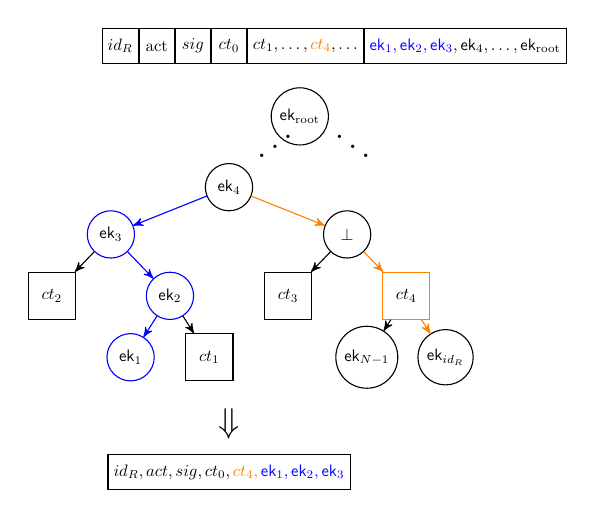
\begin{tikzpicture}[->,>=stealth',level/.style={sibling distance = 5cm/#1,
      level distance = 1.3cm},scale=0.6, transform shape,
    treenode/.style = {circle, draw=black, align=center, minimum size=1cm},
    ctnode/.style = {rectangle, draw=black, align=center, minimum size=1cm},
    packnode/.style = {rectangle, draw=black, align=center, minimum size=.75cm}]
    \tikzstyle{level 1}=[level distance=1cm]
    
    \node[packnode](pack){$id_R$};
    \node[packnode, right = 0cm of pack](pack2){act};
    \node[packnode, right = 0cm of pack2](pack3){$sig$};
    \node[packnode, right = 0cm of pack3](pack4){$ct_0$};
    \node[packnode, right = 0cm of pack4](pack5){$ct_1,\ldots, {\color{orange}ct_4}, \ldots$};
    \node[packnode, right = 0cm of pack5](pack6){${\color{blue}\mmpkepk_1,\mmpkepk_2,\mmpkepk_3},\mmpkepk_4, \ldots, \mmpkepk_{\text{root}}$};
    
    \node[below = 2.1cm of pack4, treenode](root){$\mmpkepk_4$}
    child[draw=blue]{
      node[treenode,draw=blue]{$\mmpkepk_3$}
      child[draw=black]{
        node[ctnode]{$ct_2$}
      }
      child[draw=blue]{
        node[treenode,draw=blue]{$\mmpkepk_{2}$}
        child{
          node[treenode,draw=blue]{$\mmpkepk_{1}$}
        }
        child[draw=black]{
          node[ctnode]{$ct_1$}
        }
      }
    }
    child[draw=orange]{
      node[treenode]{$\bot$}
      child[draw=black]{
        node[ctnode]{$ct_3$}
      }
      child{
        node[ctnode, draw=orange]{$ct_4$}
        child[draw=black]{
          node[treenode]{$\mmpkepk_{N-1}$}
        }
        child{
          node[treenode]{$\mmpkepk_{id_R}$}
        }
      }
    };
    \node[above right = .1cm of root](dots){\huge$\iddots$};
    \node[right = .6cm of dots]{\huge$\ddots$};
    \node[above right = 1cm of root, treenode]{$\mmpkepk_{\text{root}}$};
    \node at ($(root) + (0,-5)$)(arrow){\huge$\Downarrow$};
    \node[packnode, below = .2cm of arrow] {$id_R, act, sig, ct_0, \color{orange}{ct_4}, \color{blue}{\mmpkepk_1,\mmpkepk_2,\mmpkepk_3}$};
  \end{tikzpicture}  
  \caption{Server extraction algorithm. Lowest common ancestor (LCA) pof $id_R$ and $id_S$ is $\mmpkepk_4$, so all blue
    public keys are included in $id_R$'s packet. Since the sibling of $\mmpkepk_3$ is empty, there corresponding path
    secret of $\mmpkepk_4$ is encrypted to its resolution, resulting in the two ciphertext.
    % MM: Removed the part about c_0 since we din't use it in the main body
%    parts $ct_3$ and $ct_4$. $id_R$ can decrypt $ct_4$, since it lies on its path (orange) to the LCA . The signature and
%    header are included in every package, as well as the ciphertext-independent part ($ct_0$) of the \mmPKE encryption.
}
  \label{fig:extract-one}
\end{figure}

%%% Local Variables:
%%% mode: latex
%%% TeX-master: "main"
%%% End:


\paragraph{Comparison with techniques of \cite{hashimoto2021cmpke}.}
The work \cite{hashimoto2021cmpke} introduces a technique for efficient packet authentication which is quite similar to the technique used by \saik. In particular, their CGKA uses a committing mPKE, cmPKE. A cmPKE differs from mPKE in that encryption outputs a tag $T$ which is a cryptographic commitment to the plaintext and is delivered to each receiver. Since in \cite{hashimoto2021cmpke} every recipient of a commit gets the same message, authenticating $T$ is sufficient for CGKA authentication.
%
We highlight a couple of differences between that technique and ours:
First, it is not clear how to use cmPKE in a tree-based CGKA, where a commit executes multiple instances of \protCMPKE, and hence we end up with multiple tags $T$, each delivered to a different subset of the group.
%
Second, using the hash of the encrypted message as $T$ does not result in an IND-CCA secure \protCMPKE, since a hash allows to easily tell which of two messages is encrypted. Therefore, the construction of \cite{hashimoto2021cmpke} uses key-committing encryption to both hide and bind the message.

To summarize, \protCMPKE introduced by \cite{hashimoto2021cmpke} is very useful for the CGKA type they consider and may well find more use-cases beyond CGKA. On the other hand, \textsf{SAIK}’s solution fits all types o CGKA, does not require additional properties to prove CGKA security and is more direct. Albeit, it is very CGKA-specific.
%%% Local Variables:
%%% mode: latex
%%% TeX-master: "main"
%%% End:

% !TEX root = main.tex
% !TeX spellcheck = en_US

\section{Security of \saik}\label{sec:saik-sec-int}
To define the security we prove for \saik we fix the two safety
predicates \KwConf{} and \KwAuth{} used by $\funcCGKA$. We next give the intuition; see \cref{fig:safe} in \cref{sec:bgm_prot_proof} for the pseudocode. We define two versions of the
predicates: a stronger and a weaker one. For better exposition, the
stronger version is not achieved by \saik as presented in this work. But at the cost of added complexity
\saik can easily be extended to achieve it, as
described \cref{sec:ext-sec-predicates}.

We begin with the simpler stronger version. First, both predicates give no
guarantees for epochs in detached trees until they are attached and so we
ignore them in this section. Then, the definition is built around the notion of
secrets which make up the protocol state. There are two types of secrets:
group secrets, stored in the state of all parties, and individual secrets,
stored in the states of some parties. Each corruption exposes a number of
secrets and each epoch change replaces a number of secrets by (possibly)
secure ones. The helper predicate $\safeGrpSecsSecure{}(E)$ decides
if the group secrets in $E$ are secure, i.e., not exposed, and the
predicate $\safeIndSecsSecure(E, \id)$ decides if $\id$'s individual
secrets in $E$ are secure.
%
Then $\KwConf{}(E)$ equals to
$\safeGrpSecsSecure{}(E)$, since the epoch key is itself a group
secret. Further, $\KwAuth{}(E, \id)$ is true if either
$\safeGrpSecsSecure{}(E)$ or
$\safeIndSecsSecure(E,\id)$ is true, because both group and $\id$'s secrets
are necessary to impersonate $\id$ in $E$.

It remains to determine when group and individual secrets are exposed. For
group secrets, $\safeGrpSecsSecure(E)$ is defined recursively. The
base case states that the group secrets in first epoch (when the group was
created) are secure if and only if no party is corrupted while in that epoch.
Intuitively, we assume the group was created by an honest party using good
randomness. Moreover, capturing perfect forward secrecy, corruptions in the
descendant epochs do not affect the confidentiality of earlier group secrets.

The induction step states that the group secrets in a non-root epoch $E$
are secure if no party is corrupted in $E$, the epoch is not created
by an injected packet from the adversary and either the group secrets in
$E$'s parent $E_p$ are secure or all individual secrets in
$E$ are secure. Intuitively, this formalizes the requirement that the
adversary can learn the group secrets in only three ways: A) by corrupting a
party currently in epoch $E$. B) by injecting the secrets (though
most injections are disallowed by the authenticity predicate). C) by
computing them the same way an honest \emph{receiver} transitioning to
$E$ would. The latter requires knowing the group secrets of
$E_p$ and the individual secrets of at least one receiver. Note that
the possible receivers are those parties that are group members in
$E$ and that are not $E$'s creator (who transitions on
sending). Note also that the fact that even knowing an epoch creator's individual
secrets in $E_p$ we can treat them as secure in $E$ which captures
so called \emph{post compromise security} (aka. \emph{healing} or
\emph{backwards security}). Indeed, in \saik, part of creating a new epoch
requires refreshing all ones individual secrets.

Finally, individual secrets of $\id$ in $E$ are exposed whenever
there is some other epoch $E'$ where $\id$'s secrets are the same as
in $E$ and where $\id$ was corrupted or its secrets were injected on
its behalf. The secrets of $\id$ are the same in two epochs if no epoch between them replaces the secrets, i.e., is created by $\id$, removes
it or adds it.

\paragraph{Weaker guarantees.}
In the weaker version of the security predicates, individual secrets of $\id$
in $E$ are not secure in an additional scenario, formalized by
\safeWeakAdd. In this scenario, an $\id_s$ first honestly adds $\id$ and the
adversary $\Adv$ injects a message adding $\id$ to some other epoch. Finally,
$\id$ joins $\Adv$'s epoch and is corrupted before sending any message. We explain why \saik is insecure in this case and how it can be modified to be secure in
\cref{sec:ext-sec-predicates}.

\paragraph{Security.} 
For the \mmPKE scheme we assume a security property called \mmowrcca, defined in \cref{sec:mmowrcca}. The notion is strictly weaker than \mmindcca; in \cref{sec:mmowrcca} we prove the implication.
%
Formally, the AKS is modeled as the functionality $\funcPKI$ defined in \cref{sec:pki}. \saik
works in the $\funcPKI$-hybrids model, i.e., $\funcPKI$ is available in the real world and emulated by the simulator in the ideal world.

\newcommand{\ucideal}{\textnormal{\textsc{ideal}}}
\newcommand{\ucreal}{\textnormal{\textsc{real}}}
\begin{restatable}{theorem}{itkSec}\label{thm:saik-security}
	Let $\funcCGKA$ be the CGKA functionality with predicates \KwConf{} and \KwAuth{} defined in \cref{fig:safe}. Let $\saik$ be instantiated with an mmPKE \mmPKE, a signature scheme \sigscheme and \mac, and with the \hkdf functions modelled as a random oracle \hash.
	Let $\Adv$ be any environment. Denote the output of $\Adv$ from the real execution with \saik and the hybrid functionality $\funcPKI$ from \cref{fig:aks} as $\ucreal_{\saik, \funcPKI}(\Adv)$ and the output of $\Adv$ from the ideal execution with $\funcCGKA$ and a simulator $\ucsim$ as $\ucideal_{\funcCGKA, \ucsim}(\Adv)$.
	%
	There exists a simulator $\ucsim$ and adversaries $\Bdv[1]$ to $\Bdv[4]$ such that
	\begin{align*}
		\Pr[\ucideal&_{\funcCGKA, \ucsim}(\Adv) = 1] - \Pr\left[\ucreal_{\saik, \funcPKI}(\Adv) = 1\right] \leq \\
		&\textnormal{Adv}^{\gamefont{CR}}_{\hash}(\Bdv[1]) \\
		% confidentiality
		+\ & q_e^2(q_e+1) \log(q_n) \cdot\textnormal{Adv}^\mmowrcca_{\mmPKE,q_e\log(q_n),q_n}(\Bdv[2]) \\
		% authenticity asym
		+\ & 2q_e\cdot \textnormal{Adv}^{\ufcma}_\sigscheme(\Bdv[3]) \\
		+\ & q_e \cdot \textnormal{Adv}^{\ufcma}_\mac(\Bdv[4]) + 3q_hq_e^2(q_e+1)/2^\kappa,
	\end{align*}
	where $q_e$, $q_n$ and $q_h$ denote bounds on the number of epochs, the group size and the number of $\Adv$'s queries to the random oracle modelling the $\hash$, respectively.
	%  In the reductions, the $\hkdf$ functions are modelled as a random oracle.
  \end{restatable}

  The formal proof of \cref{thm:saik-security} can be found in \cref{sec:bgm_prot_proof}.

%%% Local Variables:
%%% mode: latex
%%% TeX-master: "main"
%%% End:

% !TEX root = main.tex
% !TeX spellcheck = en_US

\section{Evaluation}\label{sec:eval}
We compare the communication complexity or, informally, the ``bandwidth'' of \saik, \protITK and \protCMPKE from \cite{hashimoto2021cmpke}. For the sake of this comparison (and to simplify the description), one
can think of \protCMPKE as a protocol similar to \saik but where the ratchet tree is an $N$-ary tree of height $1$, where $N$ is the number of group members.
This means that \protCMPKE only needs single-message multi-recipient PKE, \mPKE (which is a special case of mmPKE).
To make a fair comparison, we instantiate \protCMPKE with the same DH-based \mPKE as \saik
instead of the less efficient but post-quantum secure \mPKE
given in \cite{hashimoto2021cmpke}.
%formulas in \cref{tab:bandwidth}.

\paragraph{Methodology.}
We compare the communication complexity of \emph{a single group modification} with respect to three metrics:
\begin{itemize}
	\item  \emph{sender bandwidth} -- the size of the packet uploaded to the
server,
\item  \emph{maximum receiver bandwidth} -- the maximum size of a (personalized) packet downloaded by a single
receiver, and
\item   \emph{total bandwidth} --  the sum of the sizes of the uploaded packet and all downloaded packets.
\end{itemize}
The sender and maximum-receiver bandwidths give an idea about the resources a single client needs to invest to perform
the group modification. In contrast, the total bandwidth gives the idea about the resources used by the server (or,
equivalently, all clients together). However, it makes no assertions about the distribution of this bandwidth, i.e. some
clients might use a significantly larger portion of the total bandwidth than others. (We note that the total bandwidth was the (only) metric used in \cite{hashimoto2021cmpke}.)

There is one caveat when calculating the bandwidth requirements for \saik (and \protITK) due to the underlying tree structure: The bandwidth can vary quite
significantly depending on the ``tree topology'', which is in turn determined by the execution history. Roughly, the reason is that add and remove operations may destroy the
good properties of the tree (by ``blanking'' nodes), increasing the number of public keys to which some message must be encrypted. In the
best case, called the \emph{tree-best-case}, there are only $\log(N)$ public keys (this happens when the ratchet has no blank nodes or unmerged
leaves, as depicted in \cref{fig:tree-full}). However, in the worst case, called the \emph{tree-worst-case}, there can be
$N$ public keys (this happens e.g. when all non-leaf nodes are blank; see \cref{fig:tree-blank}). In general, the number of public keys can be anything in between; see \cref{fig:tree-mixed}.

\begin{figure}[!tb]
  \centering
  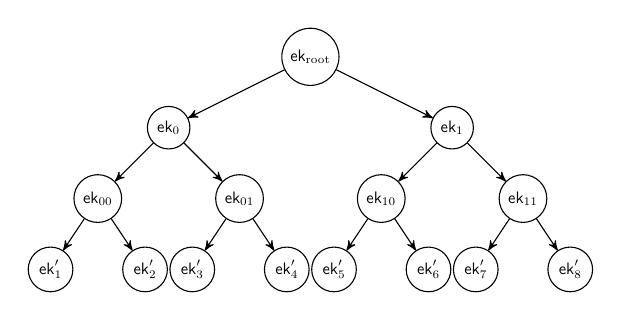
\begin{tikzpicture}[->,>=stealth',level/.style={sibling distance = 6cm/#1,
      level distance = 1.5cm},scale=0.6, transform shape,
    treenode/.style = {circle, draw=black, align=center, minimum size=.9cm}]
    
    \node[treenode](root){$\mmpkepk_{\text{root}}$}
    child{
      node[treenode]{$\mmpkepk_{0}$}
      child{
        node[treenode]{$\mmpkepk_{00}$}
        child{
          node[treenode]{$\mmpkepk'_{1}$}
        }
        child{
          node[treenode]{$\mmpkepk'_{2}$}
        }       
      }
      child{
        node[treenode]{$\mmpkepk_{01}$}
        child{
          node[treenode]{$\mmpkepk'_{3}$}
        }
        child{
          node[treenode]{$\mmpkepk'_{4}$}
        }
      }
    }
    child{
      node[treenode]{$\mmpkepk_{1}$}
      child{
        node[treenode]{$\mmpkepk_{10}$}
        child{
          node[treenode]{$\mmpkepk'_{5}$}
        }
        child{
          node[treenode]{$\mmpkepk'_{6}$}
        }       
      }
      child{
        node[treenode]{$\mmpkepk_{11}$}
        child{
          node[treenode]{$\mmpkepk'_{7}$}
        }
        child{
          node[treenode]{$\mmpkepk'_{8}$}
        }
      }
    };
  \end{tikzpicture}
  \caption{A ratchet tree for \saik or \protITK without blanks or unmerged leaves.}
  \label{fig:tree-full}
\end{figure}


\begin{figure}[!tb]
  \centering
    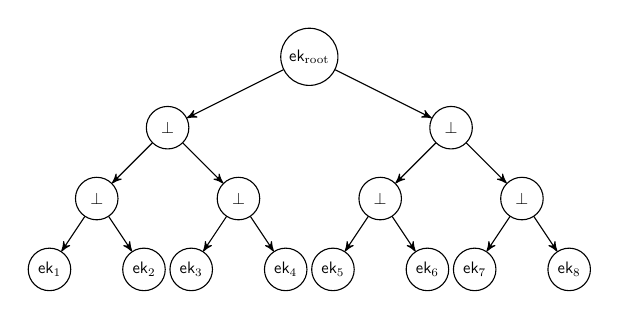
\begin{tikzpicture}[->,>=stealth',level/.style={sibling distance = 6cm/#1,
      level distance = 1.5cm},scale=0.6, transform shape,
    treenode/.style = {circle, draw=black, align=center, minimum size=.9cm}]

    \node[treenode](root){$\mmpkepk_{\text{root}}$}
    child{
      node[treenode]{$\bot$}
      child{
        node[treenode]{$\bot$}
        child{
          node[treenode]{$\mmpkepk_{1}$}
        }
        child{
          node[treenode]{$\mmpkepk_{2}$}
        }       
      }
      child{
        node[treenode]{$\bot$}
        child{
          node[treenode]{$\mmpkepk_{3}$}
        }
        child{
          node[treenode]{$\mmpkepk_{4}$}
        }
      }
    }
    child{
      node[treenode]{$\bot$}
      child{
        node[treenode]{$\bot$}
        child{
          node[treenode]{$\mmpkepk_{5}$}
        }
        child{
          node[treenode]{$\mmpkepk_{6}$}
        }       
      }
      child{
        node[treenode]{$\bot$}
        child{
          node[treenode]{$\mmpkepk_{7}$}
        }
        child{
          node[treenode]{$\mmpkepk_{8}$}
        }
      }
    };
  \end{tikzpicture}
  \caption{A ratchet tree for \saik or \protITK with all nodes blank.}
  \label{fig:tree-blank}
\end{figure}


\begin{figure}[!tb]
  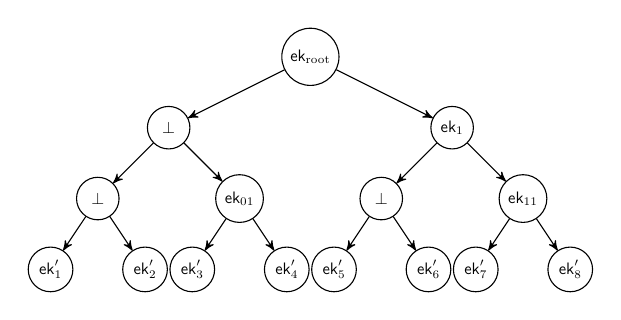
\begin{tikzpicture}[->,>=stealth',level/.style={sibling distance = 6cm/#1,
      level distance = 1.5cm},scale=0.6, transform shape,
    treenode/.style = {circle, draw=black, align=center, minimum size=.9cm}]
    
    \node[treenode](root){$\mmpkepk_{\text{root}}$}
    child{
      node[treenode]{$\bot$}
      child{
        node[treenode]{$\bot$}
        child{
          node[treenode]{$\mmpkepk'_{1}$}
        }
        child{
          node[treenode]{$\mmpkepk'_{2}$}
        }       
      }
      child{
        node[treenode]{$\mmpkepk_{01}$}
        child{
          node[treenode]{$\mmpkepk'_{3}$}
        }
        child{
          node[treenode]{$\mmpkepk'_{4}$}
        }
      }
    }
    child{
      node[treenode]{$\mmpkepk_{1}$}
      child{
        node[treenode]{$\bot$}
        child{
          node[treenode]{$\mmpkepk'_{5}$}
        }
        child{
          node[treenode]{$\mmpkepk'_{6}$}
        }       
      }
      child{
        node[treenode]{$\mmpkepk_{11}$}
        child{
          node[treenode]{$\mmpkepk'_{7}$}
        }
        child{
          node[treenode]{$\mmpkepk'_{8}$}
        }
      }
    };
  \end{tikzpicture}
  \caption{A tree with some blank and non-blank nodes. Here, sender bandwidth depends on the position in the
    tree. For example, a packet by the leftmost leaf would contain 5 ciphertexts, while the rightmost leaf would require 6.}
  \label{fig:tree-mixed}
\end{figure}

%%% Local Variables:
%%% mode: latex
%%% TeX-master: "main"
%%% End:


Therefore, we compare each bandwidth in the tree-best-case and the tree-worst-case. Note that any other case results in a bandwidth between these cases.
We remark that comparing the average over all histories of group operations would not be meaningful, since the probability of a given execution depends on user and administrator behavior, general application policies and runtime conditions, etc.
It is an important topic of future research to
better understand which kinds of policies governing when and which parties
initiate CGKA operations lead to more bandwidth efficient executions for
realistic deployments. However, it is outside the scope of this work.
%
We note that SAIK is \emph{very} flexible as to kinds of policies that are possible and the types of data that can be leveraged to guide executions towards efficient behavior. Thus, we conjecture that in practice a well designed implementation (of both server and client) will be able to ensure that under relatively mild real-time conditions the vast majority of executions will spend the overwhelming majority of their time tending towards the tree-best-case scenario in bandwidth.


\newcommand{\ctxSize}{\variable{Ctx}}
\newcommand{\mCtxSize}{\variable{mCtx}}
\newcommand{\pkSize}{\variable{Pk}}
\begin{figure*}[!p]
	\begin{minipage}[t]{\textwidth}\centering
	\begin{tabular}{|l|l|l|l|l|}
		\hline
		\multicolumn{2}{|c|}{}& \protITK & \saik & \protCMPKE \\
		\hline
		\multirow{2}{*}{Sender} 
		& tree-best-case & $\log(N)\cdot (\pkSize + \ctxSize)$ & $\log(N) \cdot \pkSize + \mCtxSize(\log(N))$ & $\pkSize + \mCtxSize(N)$ \\\cline{2-5}
		& tree-worst-case & $\log(N)\cdot\pkSize + N\cdot \ctxSize$ & $\log(N) \cdot \pkSize + \mCtxSize(N)$ & $\pkSize + \mCtxSize(N)$ \\\hline
		Maximum
		& tree-best-case & $\log(N)\cdot (\pkSize + \ctxSize)$  & $\log(N) \cdot \pkSize + \ctxSize$  & $\pkSize + \ctxSize$ \\\cline{2-5}
		receiver & tree-worst-case &  $\log(N)\cdot\pkSize + N\cdot \ctxSize$ & $\log(N) \cdot \pkSize + \ctxSize$  & $\pkSize + \ctxSize$ \\
		\hline
		\multirow{2}{*}{Total} 
		& tree-best-case & $N\log(N)\cdot (\pkSize + \ctxSize)$  & $N\log(N) \cdot \pkSize + N\cdot\ctxSize + \mCtxSize(\log(N))$   & $N\cdot(\pkSize + \ctxSize) + \mCtxSize(N)$ \\\cline{2-5}
		& tree-worst-case &  $N(\log(N)\cdot\pkSize + N\cdot \ctxSize)$ & $N\log(N) \cdot \pkSize + N\cdot\ctxSize + \mCtxSize(N)$  & $N\cdot(\pkSize + \ctxSize) + \mCtxSize(N)$ \\
		\hline
	\end{tabular}
	\caption{Sender, receiver and total bandwidth for a group of size $N$ expressed as the number of ciphertexts and public keys included in the packet (apart from this, packets include only a constant-size header).
		$\pkSize$ denotes the size of a public key (the same for PKE and mmPKE). $\mCtxSize(X)$ denotes the size of an mmPKE multi-recipient ciphertext with overall number of receivers $X$. Note that for the DH-based construction $X$ fully determines the size (i.e., it is not affected by who gets which message). $\ctxSize$ denotes the size of a PKE ciphertext, equal to the size of an individual ciphertext in the DH-based construction.
	}
	\label{tab:bandwidth1}
\end{minipage}
  \begin{minipage}[t]{.48\textwidth}
	\begin{minipage}[t]{\linewidth}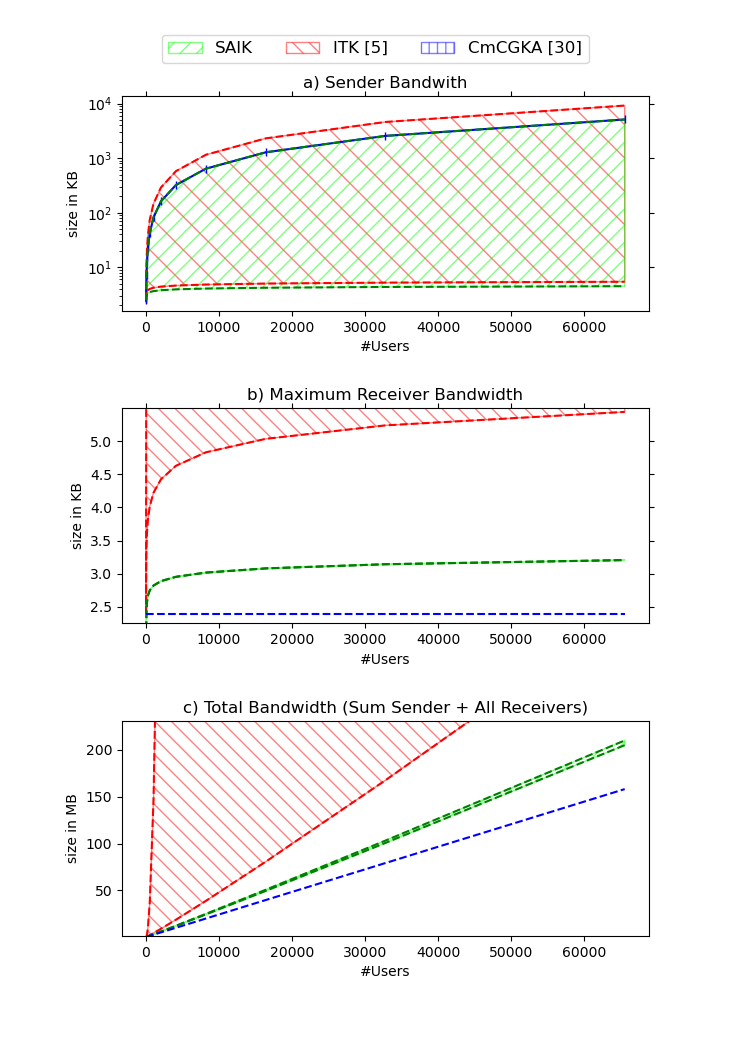
\includegraphics[width=\linewidth]{Final_Figures_Total}\end{minipage}
	\caption{Bandwidth comparison of \saik, \protITK and \protCMPKE (instantiated with 256-bit
		security). Lower lines denote the tree-best-case execution history, while upper lines denote the
		tree-worst-case. All other possible cases are marked as the regions between the lines. Plot (a) shows the sender
        bandwidth on a \emph{log scale} and plot 
		(b) shows average individual receiver bandwidth on a \emph{linear scale}. Plot (c) shows the total bandwidth,
        i.e. the sum of sender bandwidth and $n$ times the receiver bandwidth. Note that in the first plot, the lines for tree-worst-case \saik and
		all-case \protCMPKE coincide.
		%Sender and receiver bandwidth for a group of size $N$ expressed as the (approximate) number of group elements.
	}
	\label{tab:plots}
  \end{minipage}
  \hfill
  \begin{minipage}[t]{.48\textwidth}
    \centering\vspace*{-9.5cm}
    \begin{minipage}[t]{\linewidth}
    	\begin{tabular}{|l|l|l|l|l|}
    		\hline
    		\multicolumn{2}{|c|}{}& \protITK & \saik & \protCMPKE \\
    		\hline
    		\multirow{2}{*}{Sender} 
    		& best case & $3\log(N)$ & $2\log(N)$ & $N$ \\\cline{2-5}
    		& worst case &$2N$ & $N$ & $N$ \\\hline
    		\multirow{2}{*}{\parbox{1.5cm}{(Maximum)\\receiver}} 
    		& best case & $3\log(N)$ & $\log(N)$&  $3$ \\\cline{2-5}
    		& worst case & $2N$ & $\log(N)$ & $3$ \\ \hline
            \multirow{2}{*}{Total}
            & best case & $3N\log(N)$ & $N\log(N)$ & $4N $ \\\cline{2-5}
            & worst case & $2N^2$ & $N\log(N)$ & $4N$ \\
    		\hline
    	\end{tabular}
    \caption{
    	Sender, receiver and total bandwidth for a group of size $N$ expressed as the (approximate) number of group
        elements. Best/Worst case refers to the state of the tree, while we always consider the average receiver
        bandwidth over all receivers.
    }\label{fig:bandwidth2}
  \end{minipage}


  \begin{minipage}[t]{\linewidth}\centering
    \begin{tabular}{|l|r|}
      \hline
      & Bitsize \\
      \hline
      Group element & 512 \\
      \hline
      Hash & 512 \\
      \hline
      Signature & 1024 \\
      \hline
      Header & 17784 \\
      \hline
      \pkSize & 512 \\
      \hline
      \ctxSize & 1152 \\
      \hline
      $\mCtxSize(N)$ & $512 + N \cdot 640$ \\
      \hline
    \end{tabular}
    \caption{Bitsizes used to generate \cref{tab:plots}. The header consists of the sender's id, the epoch id and some
      authenticated data required by the protocol. The individual ciphertexts consist of a group element and an AEAD
      encryption, while the \mPKE ciphertext all share the same group element. The header contains signatures, tags,
      epoch and sender identifier as well as a key package. The latter makes up the bulk of the header, as it contains
      credentials, more public keys and some application data. Our estimation is based on MLS.}
    \label{tab:bits}
  \end{minipage}
  \end{minipage}
\end{figure*}
\paragraph{Results.}
We estimated the bandwidth for all protocols using the formulas in \cref{tab:bandwidth1,fig:bandwidth2} with bit lengths
indicated in \cref{tab:bits}. This is further visualized in \cref{tab:plots} for growing group sizes $N$.
We highlight some interesting observations. % features of the plots. %For concreteness, we fix $N = 10K$ users.

In terms of the sender bandwidth, \saik is always at least as good as the other protocols. 
For example, in a group of 10K parties, \saik sender's require between $83\%$ and $55\%$ of the bandwidth of \protITK (due to the smaller mmPKE ciphertexts compared to PKE). \saik's tree-worst-case sender bandwidth is the same as \protCMPKE but its tree-best-case bandwidth can be as small as $0.52\%$ by using only $4$KB in stead of \protCMPKE's $783$KB. (Recall that, unlike in \protCMPKE, in \saik sender bandwidth varies depending on the history of preceding operations.)


In terms of the maximum receiver bandwidth, \protITK is much worse than \saik and \protCMPKE. For
example, \saik receivers (at most) need between $62\%$ (tree-best-case execution) to about $.2\%$ (tree-worst-case
execution) of \protITK's. On the other hand, \protCMPKE is the best for receivers.  \saik requires up
to $126\%$ of \protCMPKE's bandwidth, i.e. an increase from $\sim 2.4$KB to $\sim 3.02$KB for 10K parties.

Finally, the total bandwidth is by far the smallest for \protCMPKE and by far the largest for \protITK. For instance,
for 10K parties, \saik requires $\sim1.3$ times more total bandwidth, while \protITK requires anywhere from $\sim2$
times (tree-best-case) to $\sim50$ times (tree-worse-case) more.

In summary, the results show that \saik achieves the lowest bandwidth required from a single client
(i.e. $\bigO(\log(N))$ for \saik vs. $\bigO(N)$ for \protCMPKE), while \protCMPKE has the lowest total bandwidth
(i.e. $\bigO(N\log(N))$ for \saik vs. $\bigO(N)$ for \protCMPKE). (Hence, both protocols meet their design goals.) For instance, for 10K parties, \protCMPKE requires a client to upload $783$KB of data, while in scenarios close to the tree-best-case (which we believe to occur most of the time), the sender or receiver bandwidth of \saik is roughly $4$KB. On the other hand, the total bandwidth is roughly $25$MB for \protCMPKE and $30$MB for \saik.

\paragraph{Server computation.}
Lastly, we consider the server-side computation for \saik and \protCMPKE. In \protCMPKE, the server only picks the
$i$-th \mPKE ciphertext for the $i$-th user and forwards all common data. For \saik, we can consider two possibilities:
Either the server keeps track of the shape of the ratchet tree (which it can do based on the header data sent in all
packages) and computes the lowest common ancestor of sender and receiver in the tree, computes its resolution and then
forwards the corresponding ciphertext and public keys. This takes at most logarithmic time in the size of the
group (however, no expensive public-key operations are required). Alternatively, the user can compute its indices in the
tree and send them to the server, reducing the server computation to effectively the same as in \protCMPKE at the cost
of an additional round of communication.

%%% Local Variables:
%%% mode: latex
%%% TeX-master: "main"
%%% End:

% !TEX root = main.tex
% !TeX spellcheck = en_US

\section{Extensions}\label{sec:extensions}
In this section we describe extensions of \saik which we did not include for simplicity.% The first extension allows to achieve slightly better security predicates at a relatively small cost. The second extension deals with primitives with imperfect correctness, such as mmPKE based on lattices.

% \subsection{Trading-off Server Computation for Communication}
% Our new (sa)CGKA \saik assumes that the mailboxing service is a full featured server capable of performing the
% individualization of messages responsible for the improved bandwidth of our protocol. This individualization mainly
% consists of generating proofs of accumulation. We assume strong accumulators which allow creation of these proofs
% without secret knowledge. However, we can trade off this server computation for increased sender communication by having the
% sender pre-compute all proofs and send them along with the rest of the packet. Receiver communication is unaffected
% by this change.

% For the hash-based accumulator described in \cref{sec:accumulators}, an easy optimization is possible. Instead of
% computing \emph{all} proofs individually, the sender can instead include the whole Huffman tree in its package. The
% server then only selects the co-paths in the tree relevant for each user, which is similarly complex to selecting the
% correct message for each user, which is exactly the task of a standard mailboxing service. This approach increases
% communication by approximately $2N$ hashes, where $N$ is the number of receiving public keys, i.e. linear in the
% number of group members in the worst case and logarithmic in the best case.

% In conclusion, our saCGKA can be transformed into a regular CGKA at the cost of sender communication while avoiding
% server computation.

% Note that the variant where each submessage is signed individually requires less communication (i.e. $N$ signatures
% instead of $2N$ hashes) than the transformed \saik variant and also doesn't require server computation. However,
% computing each signature requires an expensive public key operation, leading to a shorter sender message, but more computation for the
% sender than required by the server in \saik.

\subsection{Better Security Predicates}\label{sec:ext-sec-predicates}
We sketch the reason why \saik does not achieve the better security predicates and how it can be modified to achieve them.

Roughly, \saik achieves the worse security predicates because of the following attack: Say $\id_s$, the only corrupted party, creates a new epoch $E$ adding a new member $\id$. According to \saik, in this case $\id_s$ fetches from the Authenticated Key Service, AKS, (a type of PKI setup) a public key $\mmpkepk$ for \mmPKE and a verification key $\spk$ for \sigscheme, both registered earlier by $\id$. In epochs after $E$, parties use $\mmpkepk$ to encrypt messages to $\id$ (even before $\id$ actually joins) and $\spk$ to verify messages from $\id$. Now the adversary $\Adv$ can create a fake epoch $E'$ adding $\id$ with the same $\mmpkepk$ and $\spk$. Then, $\id$ joins $E'$ and is corrupted, leaking $\mmpkesk$ and $\ssk$. This allows $\Adv$ to compute the group key in $E$ and inject messages to parties in $E$. However, the expectation is that this is not possible, since no party is corrupted in $E$ (and $\id_s$ healed).
%
The better security predicates (formally, the predicates in \cref{fig:safe} in \cref{sec:bgm_prot_proof}) achieve just this: security in an honest epoch $E$ does not depend on whether some member joins a fake group in $E'$.

The following modification to \saik achieves better security: We note that in \saik, $\id$ registers in the AKS an additional public key $\mmpkepk'$ which is used to send secrets needed for joining. The corresponding $\mmpkesk'$ is deleted immediately after joining. In the modified \saik, when $\id_s$ adds $\id$, it generates for $\id$ new key pairs $(\mmpkepk_s,\mmpkesk_s)$ and $(\spk_s,\ssk_s)$. It sends $\mmpkesk_s$ and $\ssk_s$ to $\id$, encrypted under $\mmpkepk'$. Now messages to $\id$ are encrypted such that \emph{both} $\mmpkesk$ and $\mmpkesk_s$ are needed to decrypt them. In particular, to encrypt $m$, a sender chooses a random $r$ and encrypts $r$ under $\mmpkepk$ and $m \oplus r$ under $\mmpkepk_s$. Similarly, messages from $\id$ have two signatures, one verified under $\spk$, and one under $\spk_s$. As soon as $\id$ creates an epoch, it generates a new single \mmPKE key pair and a single \ers key pair.

The attack is prevented, because even after corrupting $\id$ in $E'$, $\Adv$ does not know $\mmpkesk'$ needed to decrypt $\mmpkesk_s$ and $\ssk_s$. Therefore, confidentiality and authenticity in $E$ is not affected.

\subsection{Primitives with Imperfect Correctness}
While the proofs of \saik security assume primitives with perfect correctness, they can be easily modified to work with
imperfect correctness. While most classically secure primitives have perfect correctness, many post-quantum
constructions (e.g. from lattices) only have statistical correctness. So this extension can be seen as a preparation for
when \saik has to be adapted to post-quantum security.

This is achieved by adding one game hop where we
abort in the new game if a correctness error occurs. This loses an additive term in the security bound that depends on
the correctness parameter and the number of possible occurrences. Additionally, the usage of primitives with imperfect
correctness generally yields imperfect correctness guarantees for the application as well (potentially with
multiplicative correctness error when using multiple primitives). For completeness, we give definitions of imperfect
correctness of the primitives used directly by \saik in this section.

\begin{definition}
We call an \mmPKE scheme \emph{$\delta$-correct}, if for all $n\in \N$, $(\mmpkepk_i,\mmpkesk_i)\in
  \mmpkeKeyGen $ for $i\in[n]$,
  $(m_1,\ldots, m_n)\in\mathcal{M}^n$ and $\forall j\in[n]$
  \[
    \Pr\left[
      \begin{array}{c}
        c_j\gets \mmpkeExt(j, C)\\
        m_j \neq \mmpkeDec(\mmpkesk_j, c_j)
      \end{array}
      \middle\vert
      C \getsr \mmpkeEnc\left(
      \begin{array}{c}
        (\mmpkepk_1,\ldots, \mmpkepk_n),\\(m_1,\ldots,m_n)
      \end{array}
      \right)
    \right] \leq \delta
  \]
\end{definition}

% \begin{definition}
%   An HRS scheme \ers for a collection of reduction pattern classes $\rdclassset_n$ for $n\in\N$ is $\delta$-correct if for all $n \in \N$, $\rdclass \in \rdclassset_n$, $(\rd,w) \in \rdclass$ and message vectors $\vec m$ of length $n$, we have
%   \begin{equation*}
%     \Pr\left[\ersvrfy\left(
%     \begin{array}{c}
%       \ersvk, k, \rd(\vec{m}),\\ \rd, \sigma'
%     \end{array}
%     \right) \neq 1
%     \middle\vert
%     \begin{array}{c}
%       (\erssk, \ersvk) \gets \erskeygen()\\
%       k \getsr \bits^\kappa\\
%       \sigma \gets \erssign(\erssk, k, \vec{m}, \rdclass) \\
%       \sigma' \gets \ersred(\ersvk, \sigma, \vec{m},\rd)
%     \end{array}
%     \right] \leq \delta.
%   \end{equation*}
% \end{definition}

% Below, we also define $\delta$-correct weighted accumulator. It is easy to see that our construction of \ers instantiated with a $\delta$-correct accumulator is also $\delta$-correct.

% \begin{definition}
%   A weighted accumulator scheme $\wacc$ is \emph{$\delta$-correct} if for every set $X$ of element-weight pairs $(x,w)$ and each $x$ s.t. $(x,\wc)\in X$, we have
%   \[
%   \Pr
%   \left[
%   \accVrfy(\accValue, x, \accProof) \neq 1
%   \middle\vert
%   \begin{array}{c}
%     (\accValue, \accaux) \getsr \accEval(X) \\
%     \accProof \getsr \accProve(\accValue, x, \accaux)
%   \end{array}
%   \right]\leq \delta.
%   \]
% \end{definition}



%%% Local Variables:
%%% mode: latex
%%% TeX-master: "main"
%%% End:


\begin{acks}
Dominik Hartmann was supported by the BMBF iBlockchain project.
Eike Kiltz was supported by the BMBF iBlockchain project, the Deutsche Forschungsgemeinschaft (DFG, German research Foundation) as part of the Excellence Strategy of the German Federal and State Governments – EXC 2092 CASA - 390781972, and by the European Union (ERC AdG REWORC - 101054911).
\end{acks}

%--- Bibliography --------------------------------------------------------------
\bibliographystyle{ACM-Reference-Format}
\balance
\bibliography{project,../cryptobib/abbrev3,../cryptobib/crypto}

\end{document}

%%% Local Variables:
%%% mode: latex
%%% TeX-master: t
%%% End:
